\documentclass{article}\usepackage[]{graphicx}\usepackage[]{color}
%% maxwidth is the original width if it is less than linewidth
%% otherwise use linewidth (to make sure the graphics do not exceed the margin)
\makeatletter
\def\maxwidth{ %
  \ifdim\Gin@nat@width>\linewidth
    \linewidth
  \else
    \Gin@nat@width
  \fi
}
\makeatother

\definecolor{fgcolor}{rgb}{0.345, 0.345, 0.345}
\newcommand{\hlnum}[1]{\textcolor[rgb]{0.686,0.059,0.569}{#1}}%
\newcommand{\hlstr}[1]{\textcolor[rgb]{0.192,0.494,0.8}{#1}}%
\newcommand{\hlcom}[1]{\textcolor[rgb]{0.678,0.584,0.686}{\textit{#1}}}%
\newcommand{\hlopt}[1]{\textcolor[rgb]{0,0,0}{#1}}%
\newcommand{\hlstd}[1]{\textcolor[rgb]{0.345,0.345,0.345}{#1}}%
\newcommand{\hlkwa}[1]{\textcolor[rgb]{0.161,0.373,0.58}{\textbf{#1}}}%
\newcommand{\hlkwb}[1]{\textcolor[rgb]{0.69,0.353,0.396}{#1}}%
\newcommand{\hlkwc}[1]{\textcolor[rgb]{0.333,0.667,0.333}{#1}}%
\newcommand{\hlkwd}[1]{\textcolor[rgb]{0.737,0.353,0.396}{\textbf{#1}}}%
\let\hlipl\hlkwb

\usepackage{framed}
\makeatletter
\newenvironment{kframe}{%
 \def\at@end@of@kframe{}%
 \ifinner\ifhmode%
  \def\at@end@of@kframe{\end{minipage}}%
  \begin{minipage}{\columnwidth}%
 \fi\fi%
 \def\FrameCommand##1{\hskip\@totalleftmargin \hskip-\fboxsep
 \colorbox{shadecolor}{##1}\hskip-\fboxsep
     % There is no \\@totalrightmargin, so:
     \hskip-\linewidth \hskip-\@totalleftmargin \hskip\columnwidth}%
 \MakeFramed {\advance\hsize-\width
   \@totalleftmargin\z@ \linewidth\hsize
   \@setminipage}}%
 {\par\unskip\endMakeFramed%
 \at@end@of@kframe}
\makeatother

\definecolor{shadecolor}{rgb}{.97, .97, .97}
\definecolor{messagecolor}{rgb}{0, 0, 0}
\definecolor{warningcolor}{rgb}{1, 0, 1}
\definecolor{errorcolor}{rgb}{1, 0, 0}
\newenvironment{knitrout}{}{} % an empty environment to be redefined in TeX

\usepackage{alltt}

% \VignetteIndexEntry{Guide to using moveHMM}
% \VignetteEngine{knitr::knitr}


\usepackage[utf8]{inputenc}
\usepackage[bf,font={small,sl}]{caption} % for pretty captions
\usepackage{natbib} % for the bibliography
\usepackage{amsmath} % for align, cases...
\usepackage{amsfonts} % for mathbb...
\usepackage{listings} % for lstlisting
\usepackage{color} % for lstlisting background color
\usepackage{booktabs} % pretty tables
\usepackage{url}
\usepackage[margin=1in]{geometry}
\usepackage{natbib}
\usepackage{comment}

\usepackage{hyperref}
\hypersetup{
    colorlinks=true,
    linkcolor=blue,
    filecolor=magenta,      
    urlcolor=cyan,
}

\urlstyle{same}

%%% the eg ie and in situ shortcuts
\newcommand{\eg}{\textit{e.g.} }
\newcommand{\ie}{\textit{i.e.} }
\newcommand{\is}{\textit{in situ} }

\title{\textbf{\texttt{HMMoce}: An R package for improved geolocation of archival‐tagged fishes using a hidden Markov method}}
\author{Camrin Braun, Ben Galuardi, Paul Gatti \& Simon Thorrold}
\IfFileExists{upquote.sty}{\usepackage{upquote}}{}
\begin{document}
\maketitle



\tableofcontents


\section{Summary}
While the number of marine animals being tagged and tracked continues to grow, current satellite tracking techniques largely constrain meaninful inference to largescale movements of surface-dwelling species and are inherently prone to significant error. Hidden Markov models (HMMs) have become increasingly common in the analysis of animal movement data by incorporating underlying behavioral states into movement data. This discretized approach also provides efficient handling of grid-based oceanographic data and likelihood surfaces generated within the package. We present an open-source \texttt{R} package, \texttt{HMMoce}, that uses a state-space HMM approach to improve position estimates derived from electronic tags using three-dimensional oceanographic data. We demonstrate \texttt{HMMoce} with example blue shark (*Prionace glauca*) data that is included in the package. Our findings illustrate how our software leverages all available tag data, along with oceanographic information, to improve position estimates of tagged marine species. For more details on these methods, including thorough references to the literature \texttt{HMMoce} is based on, please refer to \citep{Braun2018a}.

\section{Introduction}

There are many approaches to estimating animal movements from various types of tag data. The paradigm in fish tracking has been to use light levels to estimate position, but many species spend considerable time away from the photic zone. Diving behavior, like a typical diel vertical migration exhibited by deep diving swordfish, can render light geolocation useless. Yet, deep diving provides depth-temperature profile data recorded by the archival tag as it samples throughout a tagged individual's vertical movements. This sampling provides a unique signature through the oceanographic environment that can be leveraged to help constrain position. When combined with other tag-measured data streams like sea surface temperature (SST), light levels and maximum diving depth, we expect a unique combination of oceanographic characteristics to be diagnostic of an animal's location. Thus, \texttt{HMMoce} seeks to provide the framework for improving estimates of animal movements based on these oceanographic characteristics and strives to automate much of the data formatting and calculations in a transparent and flexible way.



%The analysis of animal movement data has become increasingly important in terrestrial and marine ecology. Improvements in telemetry technology have resulted in an explosion in the volume of high precision data being collected. As a result, there are two challenges which researchers collecting these data regularly face: (1) data volume and (2) employing statistical methods which can accommodate some of the specific features of movement data \citep{patterson2009}.

%A substantial part of the literature on statistical modelling of animal movement data has focused on the intuitive approach of decomposing movement time series into distinct behavioural modes (a.k.a.\ bouts, states), via the use of so-called state-switching models. These approaches typically involve assuming movements of animals to be driven by stochastically evolving states, such as a slow moving state, which may be indicative of resting or foraging, versus faster movement states which might indicate transits between foraging patches. Associated with changes in movement speeds are changes to the distribution of directional changes in the movement (known as the turning angle --- see further description below).

%Bayesian methods which employ MCMC approaches have become very popular tools for the analysis of movement data using state-switching models \citep[e.g.][]{jonsen2005, morales2004}. Typically, these have been implemented using WinBUGS \citep[although see][]{mcclintock2012}. While these models are relatively straightforward to build and hence fit in WinBUGS, the estimation can be painfully slow due to slow mixing of the MCMC samplers.

%However, for an important subset of movement data, namely highly accurate position data (e.g.\ from GPS) --- and more generally all time series of locations where the measurement error is negligible relative to the scale of the movement --- the task of statistical classification of behaviour can be done much more efficiently using hidden Markov models (HMMs) and associated frequentist inferential tools. HMMs are increasingly popular in this field, due to their flexibility and to the associated very efficient recursive algorithms available for conducting statistical inference  \citep{patterson2009, langrock2012}. The crucial requirements on movement data in order for HMMs to be suitable are that measurement error in positions is negligible and that there is a regular sampling unit (e.g.\ one positional observation per hour, or per dive, or any other meaningful unit).

\texttt{HMMoce} is an R package...% which implements HMMs and associated tools for state decoding, model selection etc.\ specifically tailored to animal movement modelling. Particular attention was paid to computational efficiency with the fitting algorithm implemented in C++. The high computational speed makes it feasible to analyze very large data sets --- e.g.\ tens of thousands of positions collected for each of a dozen individual animals --- on standard desktop PCs. The package also allows users to incorporate covariate data into their models, which is particularly useful when inferring the drivers of changes in behaviour.

%Our hope is that the \texttt{moveHMM} package will provide users who collect movement data with an interface to sophisticated and adequate methods for a statistical analysis of their data. The package is structured so as to allow the users to prepare their data for analysis, fit a variety of HMMs to their data and perform diagnostics on these fitted models.

The package is presented in %\cite{braun2018a},
where its use is illustrated on example blue and mako shark PSAT data as well as compared to other commonly employed methods for geolocation of these and similar data. A subset of the data used in that paper is included as example data in the package.

%In this vignette, we briefly introduce HMMs in the context of animal movement. We then provide a detailed example of a typical use of the package (preprocessing movement data, fitting an HMM to the data, and analyzing the fitted model). Finally, we describe more technically the structure of the package and its main functions.

\section{Example application} \label{sec:application}

%Before we provide a detailed description of the various features of the \texttt{moveHMM} package in the subsequent section, we illustrate a typical HMM-based analysis of movement data using the main functions of the package, via an example. We use the data from \cite{morales2004}, collected on four elk in Canada.

Here we illustrate the use of the package with an example dataset from a blue shark tagged with a Wildlife Computers miniPAT in the NW Atlantic. Depending on which observation likelihoods (Sec. \ref{sec:lik}) you choose to generate for your species of interest, various tag-based data streams (e.g. light, SST) may be more or less useful. Our example dataset is from a blue shark which tends to occupy the epipelagic where the tag is able to consistently record high quality light and SST data that can be used for geolocation. Furthermore, this species tends to also make daily excursions, sometimes to $>$1000 m, which yields water column temperature profiles that can also be leveraged to improve geolocation estimates. Thus, it probably makes sense to take the time to build the 3D depth-temperature likelihoods in addition to the 2D, surface-only SST, for example. For other species or behaviors, such as benthic species that rarely interact with the sea surface, a bathymetry-based likelihood is probably more appropriate and perhaps SST is less informative.

\subsection{Load and prepare the tag data} \label{sec:tag-data}

First, setup the start and end dates and locations. These are then used to build a vector of \texttt{POSIXct} timestamps that represent the desired time steps of the likelihoods and, ultimately, most probable track.

\begin{knitrout}\small
\definecolor{shadecolor}{rgb}{0.969, 0.969, 0.969}\color{fgcolor}\begin{kframe}
\begin{alltt}
\hlcom{# SET START/END LOCATIONS iniloc is dataframe containing cols: day, month,}
\hlcom{# year, lat, lon and rows: start, end}
\hlstd{iniloc} \hlkwb{<-} \hlkwd{data.frame}\hlstd{(}\hlkwd{matrix}\hlstd{(}\hlkwd{c}\hlstd{(}\hlnum{13}\hlstd{,} \hlnum{10}\hlstd{,} \hlnum{2015}\hlstd{,} \hlnum{41.3}\hlstd{,} \hlopt{-}\hlnum{69.27}\hlstd{,} \hlnum{10}\hlstd{,} \hlnum{4}\hlstd{,} \hlnum{2016}\hlstd{,} \hlnum{40.251}\hlstd{,}
    \hlopt{-}\hlnum{36.061}\hlstd{),} \hlkwc{nrow} \hlstd{=} \hlnum{2}\hlstd{,} \hlkwc{ncol} \hlstd{=} \hlnum{5}\hlstd{,} \hlkwc{byrow} \hlstd{= T))}
\hlkwd{names}\hlstd{(iniloc)} \hlkwb{<-} \hlkwd{list}\hlstd{(}\hlstr{"day"}\hlstd{,} \hlstr{"month"}\hlstd{,} \hlstr{"year"}\hlstd{,} \hlstr{"lat"}\hlstd{,} \hlstr{"lon"}\hlstd{)}
\hlstd{tag} \hlkwb{<-} \hlkwd{as.POSIXct}\hlstd{(}\hlkwd{paste}\hlstd{(iniloc[}\hlnum{1}\hlstd{,} \hlnum{1}\hlstd{],} \hlstr{"/"}\hlstd{, iniloc[}\hlnum{1}\hlstd{,} \hlnum{2}\hlstd{],} \hlstr{"/"}\hlstd{, iniloc[}\hlnum{1}\hlstd{,} \hlnum{3}\hlstd{],}
    \hlkwc{sep} \hlstd{=} \hlstr{""}\hlstd{),} \hlkwc{format} \hlstd{=} \hlstr{"%d/%m/%Y"}\hlstd{,} \hlkwc{tz} \hlstd{=} \hlstr{"UTC"}\hlstd{)}
\hlstd{pop} \hlkwb{<-} \hlkwd{as.POSIXct}\hlstd{(}\hlkwd{paste}\hlstd{(iniloc[}\hlnum{2}\hlstd{,} \hlnum{1}\hlstd{],} \hlstr{"/"}\hlstd{, iniloc[}\hlnum{2}\hlstd{,} \hlnum{2}\hlstd{],} \hlstr{"/"}\hlstd{, iniloc[}\hlnum{2}\hlstd{,} \hlnum{3}\hlstd{],}
    \hlkwc{sep} \hlstd{=} \hlstr{""}\hlstd{),} \hlkwc{format} \hlstd{=} \hlstr{"%d/%m/%Y"}\hlstd{,} \hlkwc{tz} \hlstd{=} \hlstr{"UTC"}\hlstd{)}

\hlcom{# VECTOR OF DATES FROM DATA. THIS WILL BE THE TIME STEPS, T, IN THE}
\hlcom{# LIKELIHOODS}
\hlstd{dateVec} \hlkwb{<-} \hlkwd{seq.POSIXt}\hlstd{(tag, pop,} \hlkwc{by} \hlstd{=} \hlstr{"24 hours"}\hlstd{)}
\end{alltt}
\end{kframe}
\end{knitrout}

\subsubsection{Sea surface temperature data}

Next, we load some tag data. Raw example data is included with the package and can be read by pointing to the "extdata" directory associated with the install of the \texttt{HMMoce} package. Helper functions are provided for directly reading data from Wildlife Computers tags, however \texttt{HMMoce} works with any tag data that can be coerced to the minimum required input data for the various observation likelihoods. Over time, these have been generalized from WC-specific to more flexible implementations for use with other manufacturers. The minimum required SST data for use in \texttt{HMMoce}, and thus the output from the WC helper function, is "Date", "Depth", and "Temperature". Date must be of class POSIXct. Depth represents the depth at which the corresponding sea surface temperature ("Temperature") was taken. These data requirements are easily fulfilled when working with other tag types (e.g. daily max temperature from Microwave X-tag). Currently the column "Depth" is not used but is retained here for user convenience in case, for example, it makes sense to filter the SST data due to SSTs being recorded deeper than what makes sense given the oceanography the tagged animal is in. 

\begin{knitrout}\small
\definecolor{shadecolor}{rgb}{0.969, 0.969, 0.969}\color{fgcolor}\begin{kframe}
\begin{alltt}
\hlstd{sstFile} \hlkwb{<-} \hlkwd{system.file}\hlstd{(}\hlstr{"extdata"}\hlstd{,} \hlstr{"141259-SST.csv"}\hlstd{,} \hlkwc{package} \hlstd{=} \hlstr{"HMMoce"}\hlstd{)}
\hlstd{tag.sst} \hlkwb{<-} \hlkwd{read.wc}\hlstd{(sstFile,} \hlkwc{type} \hlstd{=} \hlstr{"sst"}\hlstd{,} \hlkwc{tag} \hlstd{= tag,} \hlkwc{pop} \hlstd{= pop,} \hlkwc{verbose} \hlstd{= F)}
\hlstd{tag.sst} \hlkwb{<-} \hlstd{tag.sst[,} \hlkwd{c}\hlstd{(}\hlstr{"Date"}\hlstd{,} \hlstr{"Depth"}\hlstd{,} \hlstr{"Temperature"}\hlstd{)]}
\hlkwd{head}\hlstd{(tag.sst)}
\end{alltt}
\begin{verbatim}
                 Date Depth Temperature
1 2015-10-14 10:00:00     0        15.1
2 2015-10-15 10:00:00     0        14.6
3 2015-10-16 05:00:00     0        14.7
4 2015-10-17 07:00:00     0        14.2
5 2015-10-18 03:00:00     0        14.6
6 2015-10-19 09:00:00     0        13.6
\end{verbatim}
\end{kframe}
\end{knitrout}

\subsubsection{Depth-temperature data}

Next is some representation of water column structure. There are many options here based on tag model, animal behavior, etc. but ultimately the goal is to create a tag-based dataset that represents the thermal structure of the water column and contains columns at least for: "Date" (again POSIXct), "Depth", "MinTemp", and "MaxTemp". A fifth column called "MeanTemp" can be included which will be used as the temperature for likelihood construction. If "MeanTemp" doesn't exist, \texttt{HMMoce} will by default calculate the midpoint between min and max temperature for each measurement and use that for subsequent calculations.

By comparing tag-recorded thermal structure to the oceanographic environment, we can often add a very rich set of information for geolocation. For example, a tag sampling the thermal structure of the Sargasso Sea would yield very different results from that of the Gulf Stream or Labrador Sea \citep[\eg basking sharks][]{Braun2018b}. Tags like the example miniPAT used here provide summaries of depth-temperature profiles as a .csv called "-PDTs" for which there's a helper function.

\begin{knitrout}\small
\definecolor{shadecolor}{rgb}{0.969, 0.969, 0.969}\color{fgcolor}\begin{kframe}
\begin{alltt}
\hlcom{# DEPTH-TEMPERATURE PROFILE DATA example is output from Wildlife Computer}
\hlcom{# Portal pdt needs to contain at least: - Date (POSIXct) - Depth - MinTemp -}
\hlcom{# MaxTemp - MeanTemp (optional): if meantemp doesn't exist for whatever}
\hlcom{# reason, HMMoce will calculate the midpoint between min/max temps and use}
\hlcom{# that}

\hlstd{pdtFile} \hlkwb{<-} \hlkwd{system.file}\hlstd{(}\hlstr{"extdata"}\hlstd{,} \hlstr{"141259-PDTs.csv"}\hlstd{,} \hlkwc{package} \hlstd{=} \hlstr{"HMMoce"}\hlstd{)}
\hlstd{pdt} \hlkwb{<-} \hlkwd{read.wc}\hlstd{(pdtFile,} \hlkwc{type} \hlstd{=} \hlstr{"pdt"}\hlstd{,} \hlkwc{tag} \hlstd{= tag,} \hlkwc{pop} \hlstd{= pop,} \hlkwc{verbose} \hlstd{= F)}
\hlstd{pdt} \hlkwb{<-} \hlstd{pdt[,} \hlkwd{c}\hlstd{(}\hlstr{"Date"}\hlstd{,} \hlstr{"Depth"}\hlstd{,} \hlstr{"MinTemp"}\hlstd{,} \hlstr{"MaxTemp"}\hlstd{)]}
\hlkwd{head}\hlstd{(pdt)}
\end{alltt}
\begin{verbatim}
          Date Depth MinTemp MaxTemp
1   2015-10-14     0    14.2    16.0
96  2015-10-14     8    13.6    16.0
191 2015-10-14    24    12.2    15.6
286 2015-10-14    48     9.8    14.4
2   2015-10-15     0    14.6    16.6
97  2015-10-15     8    14.6    16.6
\end{verbatim}
\end{kframe}
\end{knitrout}

Depending on tag type, there are many ways to represent this vertical structure. For example, miniPATs can also report summaries of depth-temperature time series which could be used to re-construct custom depth-temperature profiles. Similarly, other models such as the Microwave X-tag or various archival tags from Wildlife Computers or Lotek report high-resolution time series of depth and temperature. These can be used to construct custom depth-temperature profiles. A few things to keep in mind for building custom summaries of this type of data:
\begin{itemize}
\item vertical depth levels are ultimately compared to whatever depth levels are available in the environmental dataset you compare to for building likelihoods. Thus, it might make sense to make your custom depth levels match, for example, the HYCOM depth levels you will compare the tag data to
\item temporal resolution of your summarized dataset can only be as high as the resolution of your `dateVec` object that is the "temporal backbone" of this entire modeling process. Thus, it makes sense that the timescales and resolution of these match as much as possible.
\end{itemize}

The example below shows HMMoce functionality for coercing time series data to depth-temperature summary data using transmitted data from the example miniPAT; however, a similar approach can be used for time series from other tags. Note that the resulting data from this reformatting matches the format of the depth-temperature output above as we're assuming these are equivalent data products. Only one of these is necessary for subsequent likelihood construction. Due to data transmission constraints, it is usually best to use the summarized data for tags that report them (e.g. miniPAT), but constructing custom summaries like this can be useful for certain situations and are necessary for datasets that only have time series (e.g. archival tags).

\begin{knitrout}\small
\definecolor{shadecolor}{rgb}{0.969, 0.969, 0.969}\color{fgcolor}\begin{kframe}
\begin{alltt}
\hlcom{# DEPTH-TEMPERATURE TIME SERIES DATA exampling showing how to coerce}
\hlcom{# depth-temp time series to a PDT-like summarized product}

\hlstd{tsFile} \hlkwb{<-} \hlkwd{system.file}\hlstd{(}\hlstr{"extdata"}\hlstd{,} \hlstr{"141259-Series.csv"}\hlstd{,} \hlkwc{package} \hlstd{=} \hlstr{"HMMoce"}\hlstd{)}
\hlcom{## bandaid to access the series data without installing new HMMoce}
\hlstd{tsFile} \hlkwb{<-} \hlstr{"~/work/RCode/HMMoce/inst/extdata/141259-Series.csv"}
\hlstd{ts} \hlkwb{<-} \hlkwd{read.table}\hlstd{(tsFile,} \hlkwc{sep} \hlstd{=} \hlstr{","}\hlstd{,} \hlkwc{header} \hlstd{= T)}
\hlstd{ts}\hlopt{$}\hlstd{Date} \hlkwb{<-} \hlkwd{as.POSIXct}\hlstd{(}\hlkwd{paste}\hlstd{(ts}\hlopt{$}\hlstd{Day, ts}\hlopt{$}\hlstd{Time),} \hlkwc{format} \hlstd{=} \hlstr{"%d-%b-%Y %H:%M:%S"}\hlstd{,}
    \hlkwc{tz} \hlstd{=} \hlstr{"UTC"}\hlstd{)}
\hlstd{ts} \hlkwb{<-} \hlstd{ts[,} \hlkwd{c}\hlstd{(}\hlstr{"Date"}\hlstd{,} \hlstr{"Depth"}\hlstd{,} \hlstr{"Temperature"}\hlstd{)]}

\hlcom{## generate depth-temp summary from time series}
\hlstd{pdt} \hlkwb{<-} \hlkwd{bin_TempTS}\hlstd{(ts,} \hlkwc{out_dates} \hlstd{= dateVec,} \hlkwc{bin_res} \hlstd{=} \hlnum{25}\hlstd{)}
\hlstd{pdt} \hlkwb{<-} \hlstd{pdt[,} \hlkwd{c}\hlstd{(}\hlstr{"Date"}\hlstd{,} \hlstr{"Depth"}\hlstd{,} \hlstr{"MinTemp"}\hlstd{,} \hlstr{"MaxTemp"}\hlstd{)]}
\hlkwd{head}\hlstd{(pdt)}
\end{alltt}
\begin{verbatim}
        Date Depth MinTemp MaxTemp
1 2015-10-15     0   15.35   15.50
2 2015-10-15    25   14.30   15.35
3 2015-10-15    50   12.75   13.75
4 2015-10-15    75   10.17   10.17
5 2015-10-19     0   13.66   13.71
6 2015-10-19    25   13.69   14.11
\end{verbatim}
\end{kframe}
\end{knitrout}


\subsubsection{Light data} \label{sec:light-data}

Light data has been at the core of geolocation estimates in marine and terrestrial environments for decades (hill ref). As such, there are a number of methods for using tag-based light measurements to generate likelihoods of where on Earth those light measurements were recorded. Taking light measurements from the back of a marine animal can be particularly error-prone as that animal is moving through a range of turbid to clear water, diving from the photic zone to great depths, and at least indirectly experiencing cloud cover and many other factors that can affect light measurements. Here, we focus on two main types of light data one might get from an archival tag in the marine environment: raw light levels and light-based position estimates. This can be an important distinction when building likelihoods based on light (Sec. \ref{sec:lik}).

\vspace{2mm}
\noindent \textbf{"Raw" light data}

\noindent Raw light curves and/or sunrise and sunset times are recorded by most (if not all) archival tags. Our example miniPAT contains raw light curves but onboard processing has already determined sunrise and sunset times for us. If you go this route, required columns are "Date" (POSIXct) and "Type" where only "Dawn" and "Dusk" are recognized as valid types corresponding to sunrise and sunset, respectively.
\begin{knitrout}\small
\definecolor{shadecolor}{rgb}{0.969, 0.969, 0.969}\color{fgcolor}\begin{kframe}
\begin{alltt}
\hlstd{lightFile} \hlkwb{<-} \hlkwd{system.file}\hlstd{(}\hlstr{"extdata"}\hlstd{,} \hlstr{"141259-LightLoc.csv"}\hlstd{,} \hlkwc{package} \hlstd{=} \hlstr{"HMMoce"}\hlstd{)}
\hlstd{light} \hlkwb{<-} \hlkwd{read.wc}\hlstd{(lightFile,} \hlkwc{type} \hlstd{=} \hlstr{"light"}\hlstd{,} \hlkwc{tag} \hlstd{= tag,} \hlkwc{pop} \hlstd{= pop,} \hlkwc{verbose} \hlstd{= F)}
\hlcom{## combine character vectors 'Day' and 'Time' to generate POSIXct object}
\hlstd{light}\hlopt{$}\hlstd{Date} \hlkwb{<-} \hlstd{lubridate}\hlopt{::}\hlkwd{dmy_hms}\hlstd{(}\hlkwd{paste}\hlstd{(light}\hlopt{$}\hlstd{Day, light}\hlopt{$}\hlstd{Time,} \hlkwc{sep} \hlstd{=} \hlstr{" "}\hlstd{))}
\hlstd{light} \hlkwb{<-} \hlstd{light[,} \hlkwd{c}\hlstd{(}\hlstr{"Date"}\hlstd{,} \hlstr{"Type"}\hlstd{)]}
\end{alltt}
\end{kframe}
\end{knitrout}

Our example miniPAT looks like this:

\begin{knitrout}\small
\definecolor{shadecolor}{rgb}{0.969, 0.969, 0.969}\color{fgcolor}\begin{kframe}
\begin{alltt}
\hlkwd{head}\hlstd{(light)}
\end{alltt}
\begin{verbatim}
                  Date Type
5  2015-10-15 09:56:15 Dawn
6  2015-10-15 21:52:30 Dusk
7  2015-10-16 09:45:00 Dawn
8  2015-10-16 21:50:00 Dusk
9  2015-10-17 09:57:30 Dawn
10 2015-10-17 21:48:45 Dusk
\end{verbatim}
\end{kframe}
\end{knitrout}

Similar measurements are taken by nearly every other archival or pop-up tag we're aware of and can thus be coerced to the same format as above.

\vspace{2mm}
\noindent \textbf{Light-based position estimates}

Many models of archival tag require manufacturer-specific post-processing which often generates light-based position estimates. These estimates often result in more realistic light-based likelihoods and are thus recommended over the "raw" light approach above. To incorporate light-based position estimates into the likelihood process, required columns are "Date" (POSIXct), estimated "Longitude", and "Error.Semi.minor.axis" which represents the error/uncertainty in the longitude estimate in METERS(!). With only these columns, you can generate longitude-only light-based likelihoods (i.e. if latitude estimates are unreliable and thus uninformative). To include latitude information and thus generate elliptical light-based likelihoods, the following additional columns are required: "Latitude", "Error.Semi.major.axis" (again, in meters), "Offset" (shift the ellipse this distance in METERS), "Offset.orientation" (currently 0 for North and 180 for South, no other orientation angles are currently supported). If your manufacturer didn't provide offset values, use 0 for both.
\begin{knitrout}\small
\definecolor{shadecolor}{rgb}{0.969, 0.969, 0.969}\color{fgcolor}\begin{kframe}
\begin{alltt}
\hlcom{# LIGHT BASED POSITIONS FROM GPE2 (INSTEAD OF RAW LIGHTLOCS FROM PREVIOUS)}
\hlstd{llFile} \hlkwb{<-} \hlkwd{system.file}\hlstd{(}\hlstr{"extdata"}\hlstd{,} \hlstr{"141259-Locations-GPE2.csv"}\hlstd{,} \hlkwc{package} \hlstd{=} \hlstr{"HMMoce"}\hlstd{)}
\hlstd{lightloc} \hlkwb{<-} \hlkwd{read.table}\hlstd{(llFile,} \hlkwc{sep} \hlstd{=} \hlstr{","}\hlstd{,} \hlkwc{header} \hlstd{= T,} \hlkwc{blank.lines.skip} \hlstd{= F)}
\hlstd{lightloc} \hlkwb{<-} \hlstd{lightloc[}\hlkwd{which}\hlstd{(lightloc}\hlopt{$}\hlstd{Type} \hlopt{!=} \hlstr{"Argos"}\hlstd{), ]}
\hlstd{lightloc} \hlkwb{<-} \hlstd{lightloc[,} \hlkwd{c}\hlstd{(}\hlstr{"Date"}\hlstd{,} \hlstr{"Longitude"}\hlstd{,} \hlstr{"Error.Semi.minor.axis"}\hlstd{,} \hlstr{"Latitude"}\hlstd{,}
    \hlstr{"Error.Semi.major.axis"}\hlstd{,} \hlstr{"Offset"}\hlstd{,} \hlstr{"Offset.orientation"}\hlstd{)]}
\hlstd{lightloc}\hlopt{$}\hlstd{Date} \hlkwb{<-} \hlkwd{as.POSIXct}\hlstd{(lightloc}\hlopt{$}\hlstd{Date,} \hlkwc{format} \hlstd{=} \hlkwd{findDateFormat}\hlstd{(lightloc}\hlopt{$}\hlstd{Date))}
\hlkwd{head}\hlstd{(lightloc)}
\end{alltt}
\begin{verbatim}
                 Date Longitude Error.Semi.minor.axis Latitude
1 2015-10-14 10:28:45 -68.20703                 71078     42.5
2 2015-10-14 22:36:15 -68.83478                 58991     45.0
3 2015-10-15 22:26:15 -68.13254                 16835     49.0
4 2015-10-16 10:18:45 -68.86938                 46343     45.0
5 2015-10-16 22:23:45 -68.65265                 27293     41.5
6 2015-10-17 10:31:15 -68.34464                 38261     45.5
  Error.Semi.major.axis Offset Offset.orientation
1               1583460 611160                  0
2               1527900 611160                  0
3               1416780 500040                  0
4               1277880 333360                  0
5                972300 277800                  0
6               1111200 222240                  0
\end{verbatim}
\end{kframe}
\end{knitrout}



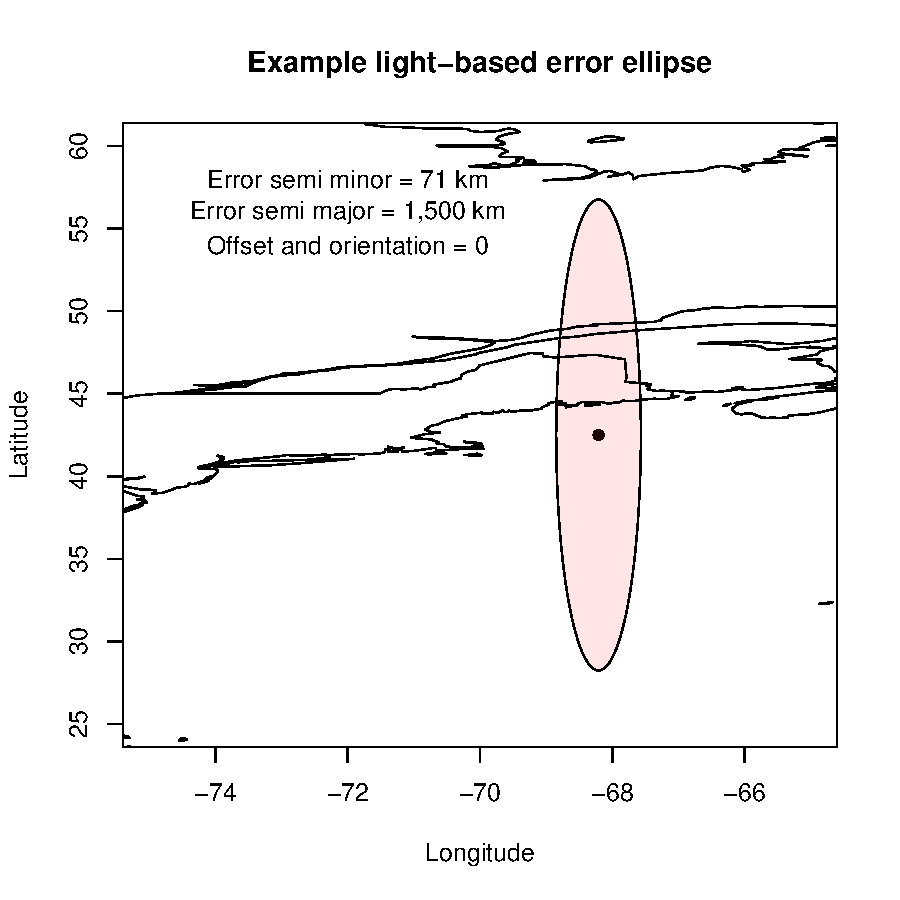
\includegraphics[width=5in, keepaspectratio]{./light_ell.pdf}

The column names above are derived from Wildlife Computers outputs but data from other manufacturers can be readily coerced to match this format. For example, Microwave Telemetry provides estimated latitude/longitude values based on their proprietary post-processing methods (in 'Lat\&Long' sheet in an x-tag report). Since these aren't provided with error estimates, we can use empirical error estimates fixed at 0.7$^\circ$ longitude following \cite{Musyl2011} (although note that such error seems rather generous and is likely higher).

\begin{knitrout}\small
\definecolor{shadecolor}{rgb}{0.969, 0.969, 0.969}\color{fgcolor}\begin{kframe}
\begin{alltt}
\hlstd{MWTdata}  \hlcom{## from Lat&Long sheet from x-tag}
\hlkwd{names}\hlstd{(MWTdata)} \hlkwb{=} \hlkwd{c}\hlstd{(}\hlstr{"Date"}\hlstd{,} \hlstr{"Latitude"}\hlstd{,} \hlstr{"Longitude"}\hlstd{)}
\hlcom{## set fixed longitude error estimate in METERS}
\hlstd{MWTdata}\hlopt{$}\hlstd{Error.Semi.minor.axis} \hlkwb{=} \hlnum{0.7} \hlopt{*} \hlnum{1000} \hlopt{*} \hlnum{111}
\end{alltt}
\end{kframe}
\end{knitrout}

\subsubsection{Depth-only data} \label{sec:depth-data}

Most archival tags collect data on depth and many report statistics for depth, such as min and max, over a given summary period. It can often be useful to use at least the maximum depth over, for example, each day of a deployment to inform geolocation estimates. For benthic or bottom-oriented species, we can leverage both the max and min depths to constrain an animal's possible movements. To do this, we need some kind of summary of the depth data.

Our example miniPAT reports a summary sheet that already contains these values:

\begin{knitrout}\small
\definecolor{shadecolor}{rgb}{0.969, 0.969, 0.969}\color{fgcolor}\begin{kframe}
\begin{alltt}
\hlstd{mmdFile} \hlkwb{<-} \hlkwd{system.file}\hlstd{(}\hlstr{"extdata"}\hlstd{,} \hlstr{"141259-MinMaxDepth.csv"}\hlstd{,} \hlkwc{package} \hlstd{=} \hlstr{"HMMoce"}\hlstd{)}
\hlstd{mmd} \hlkwb{<-} \hlkwd{read.table}\hlstd{(mmdFile,} \hlkwc{sep} \hlstd{=} \hlstr{","}\hlstd{,} \hlkwc{header} \hlstd{= T,} \hlkwc{blank.lines.skip} \hlstd{= F)[,} \hlkwd{c}\hlstd{(}\hlstr{"Date"}\hlstd{,}
    \hlstr{"MinDepth"}\hlstd{,} \hlstr{"MaxDepth"}\hlstd{)]}
\hlstd{mmd}\hlopt{$}\hlstd{Date} \hlkwb{<-} \hlkwd{as.POSIXct}\hlstd{(mmd}\hlopt{$}\hlstd{Date,} \hlkwc{format} \hlstd{=} \hlkwd{findDateFormat}\hlstd{(mmd}\hlopt{$}\hlstd{Date))}
\hlkwd{head}\hlstd{(mmd)}
\end{alltt}
\begin{verbatim}
        Date MinDepth MaxDepth
1 2015-10-13    0.375       51
2 2015-10-14    0.000       48
3 2015-10-15    0.000       88
4 2015-10-16    0.000       56
5 2015-10-17   16.000       16
6 2015-10-18    0.000       16
\end{verbatim}
\end{kframe}
\end{knitrout}

However, given a depth time series data stream from your tag, which is far more common, it is trivial to generate your own custom depth summary statistics. The benefit of the latter approach is full control over the temporal resolution of the summary if, for example, you wanted to generate likelihoods at finer timesteps than the onboard processing of depth summary statistics would allow.

\begin{knitrout}\small
\definecolor{shadecolor}{rgb}{0.969, 0.969, 0.969}\color{fgcolor}\begin{kframe}
\begin{alltt}
\hlstd{seriesFile} \hlkwb{<-} \hlkwd{system.file}\hlstd{(}\hlstr{"extdata"}\hlstd{,} \hlstr{"141259-Series.csv"}\hlstd{,} \hlkwc{package} \hlstd{=} \hlstr{"HMMoce"}\hlstd{)}
\hlstd{series} \hlkwb{<-} \hlkwd{read.table}\hlstd{(seriesFile,} \hlkwc{sep} \hlstd{=} \hlstr{","}\hlstd{,} \hlkwc{header} \hlstd{= T,} \hlkwc{blank.lines.skip} \hlstd{= F)[,}
    \hlkwd{c}\hlstd{(}\hlstr{"Day"}\hlstd{,} \hlstr{"Time"}\hlstd{,} \hlstr{"Depth"}\hlstd{,} \hlstr{"Temperature"}\hlstd{)]}
\hlstd{series}\hlopt{$}\hlstd{Date} \hlkwb{<-} \hlkwd{as.Date}\hlstd{(}\hlkwd{as.POSIXct}\hlstd{(}\hlkwd{paste}\hlstd{(series}\hlopt{$}\hlstd{Day, series}\hlopt{$}\hlstd{Time),} \hlkwc{format} \hlstd{=} \hlstr{"%d-%b-%Y %H:%M:%S"}\hlstd{,}
    \hlkwc{tz} \hlstd{=} \hlstr{"UTC"}\hlstd{))}
\hlstd{mmd} \hlkwb{<-} \hlstd{series} \hlopt \hlkwd{group_by}\hlstd{(Date)} \hlopt \hlstd{dplyr}\hlopt{::}\hlkwd{summarise}\hlstd{(}\hlkwc{n} \hlstd{=} \hlkwd{n}\hlstd{(),} \hlkwc{MinDepth} \hlstd{=} \hlkwd{min}\hlstd{(Depth,}
    \hlkwc{na.rm} \hlstd{= T),} \hlkwc{MaxDepth} \hlstd{=} \hlkwd{max}\hlstd{(Depth,} \hlkwc{na.rm} \hlstd{= T),} \hlkwc{.groups} \hlstd{=} \hlstr{"keep"}\hlstd{)}
\hlkwd{head}\hlstd{(mmd)}
\end{alltt}
\begin{verbatim}
# A tibble: 6 x 4
# Groups:   Date [6]
  Date           n MinDepth MaxDepth
  <date>     <int>    <dbl>    <dbl>
1 2015-10-13   219      0.5     51  
2 2015-10-14   240      0.5     34.5
3 2015-10-15   480      0.5     80  
4 2015-10-16    48      2.5     17  
5 2015-10-17    96      0.5     26.5
6 2015-10-19   432      0.5     51  
\end{verbatim}
\end{kframe}
\end{knitrout}

\subsection{Environmental data} \label{sec:env}

Now that the tag data is prepared, the next major step is to acquire all the necessary environmental data to compare the tag data to. Depending on which likelihoods you choose to build, the required environmental data will vary. Light-based likelihoods require no environmental data as the spatial variation in sunrise and sunset times are known.

\subsubsection{Spatial limits}
First, establish the spatial bounds of this model run. How you do this can vary widely based on species, their movement ecology, and the quality of the tag data used. This step is \textbf{critical} in the model setup because it \textbf{must} incorporate the complete geographic limits of your animal(s) movements! These limits are used for downloading environmental data and, ultimately, serve as the bounds for the model. Thus, err on the side of making the bounds too large to be sure the extent of movements are adequately captured. If they aren't, the estimated movements will likely run into the edges of your spatial limits (specified here), and you will have to start over. The tradeoff as model bounds expand is, of course, computational demands increase as larger grids are computed. In the end, the choice of spatial bounds comes down to expert opinion so choose carefully.

This step is typically accomplished best by a combination of expert opinion (thats you!) and by looking at the spatial bounds of tagging and pop-up locations and longitude estimates (if you have them). If you don't have position estimates to start with, do some preliminary plotting of tag data (such as SST) to try to constrain where you think the animal went. There's no harm in having to come back to this when your model runs into the boundaries except that you'll have to download all the environmental data again which, you will soon find out, takes time. To that end, be smart about setting spatial limits when you plan to analyze data for a group of tag datasets. Find the largest common grid and use that for all analyses. That means you only have to download the oceanographic data once!

Here, we set our bounds over a large portion of the NW Atlantic as blue sharks are known to be highly migratory, and this individual could easily cover much of this area over the duration of the tag deployment. This decision was ultimately made by comparing the tag and pop-up locations to the depth-temperature information recorded onboard the tag to explore the likely water masses the animal encountered and thus the extent of movement.

\begin{knitrout}\small
\definecolor{shadecolor}{rgb}{0.969, 0.969, 0.969}\color{fgcolor}\begin{kframe}
\begin{alltt}
\hlcom{# SET SPATIAL LIMITS these are the lat/lon bounds of your study area (e.g.}
\hlcom{# where you think the animal went)}
\hlstd{sp.lim} \hlkwb{<-} \hlkwd{list}\hlstd{(}\hlkwc{lonmin} \hlstd{=} \hlopt{-}\hlnum{80}\hlstd{,} \hlkwc{lonmax} \hlstd{=} \hlopt{-}\hlnum{25}\hlstd{,} \hlkwc{latmin} \hlstd{=} \hlnum{15}\hlstd{,} \hlkwc{latmax} \hlstd{=} \hlnum{50}\hlstd{)}

\hlcom{## setup the spatial grid to base likelihoods on}
\hlstd{locs.grid} \hlkwb{<-} \hlkwd{setup.locs.grid}\hlstd{(sp.lim,} \hlkwc{res} \hlstd{=} \hlstr{"quarter"}\hlstd{)}
\end{alltt}
\end{kframe}
\end{knitrout}

If you plan to analyze multiple tag datasets over a similar time period and spatial domain, consider that before downloading the environmental datasets to save yourself from having to change spatial/temporal bounds later and download everything again. For a group of tags, combine the unique dates and expected spatial bounds across all tags to find a common spatial extent before downloading the environmental data (e.g. SST).

\subsubsection{SST data}

There are a number of SST products out there that meet our needs. While modeled SST products work fine, we typically use remote-sensing products. There are 3 products currently built into the \texttt{get.env} functionality within \texttt{HMMoce} (see \texttt{?get.env}). Here we'll use the Optimum Interpolation SST (OISST) from NOAA. Note the tradeoffs associated with different SST products such as gaps, gap-filling techniques/interpolations, product resolution and temporal coverage/availability of a given product. Here we get one file as an example:

\begin{knitrout}\small
\definecolor{shadecolor}{rgb}{0.969, 0.969, 0.969}\color{fgcolor}\begin{kframe}
\begin{alltt}
\hlcom{## here we get use a ridculously small spatial extent for this species, just}
\hlcom{## to show some example environmental data}
\hlstd{udates} \hlkwb{<-} \hlkwd{seq.Date}\hlstd{(}\hlkwd{as.Date}\hlstd{(tag),} \hlkwd{as.Date}\hlstd{(pop),} \hlkwc{by} \hlstd{=} \hlstr{"day"}\hlstd{)}
\hlstd{sst.dir} \hlkwb{<-} \hlkwd{paste0}\hlstd{(dir,} \hlstr{"/EnvData/sst/"}\hlstd{)}
\hlkwa{if} \hlstd{(}\hlopt{!}\hlkwd{dir.exists}\hlstd{(sst.dir))} \hlkwd{dir.create}\hlstd{(sst.dir,} \hlkwc{recursive} \hlstd{=} \hlnum{TRUE}\hlstd{)}
\hlkwa{if} \hlstd{(}\hlopt{!}\hlkwd{file.exists}\hlstd{(}\hlkwd{paste0}\hlstd{(sst.dir,} \hlstr{"oisst_"}\hlstd{, udates[}\hlnum{1}\hlstd{],} \hlstr{".nc"}\hlstd{)))} \hlkwd{get.env}\hlstd{(udates[}\hlnum{1}\hlstd{],}
    \hlkwc{filename} \hlstd{=} \hlstr{"oisst"}\hlstd{,} \hlkwc{type} \hlstd{=} \hlstr{"sst"}\hlstd{,} \hlkwc{sst.type} \hlstd{=} \hlstr{"oi"}\hlstd{,} \hlkwc{spatLim} \hlstd{= sp.lim,} \hlkwc{save.dir} \hlstd{= sst.dir)}

\hlstd{sst} \hlkwb{<-} \hlstd{raster}\hlopt{::}\hlkwd{raster}\hlstd{(}\hlkwd{paste0}\hlstd{(sst.dir,} \hlstr{"oisst_"}\hlstd{, udates[}\hlnum{1}\hlstd{],} \hlstr{".nc"}\hlstd{))}
\hlkwd{plot}\hlstd{(sst,} \hlkwc{main} \hlstd{=} \hlstr{"Example SST field"}\hlstd{)}
\hlkwd{world}\hlstd{(}\hlkwc{add} \hlstd{= T)}
\end{alltt}
\end{kframe}
\end{knitrout}

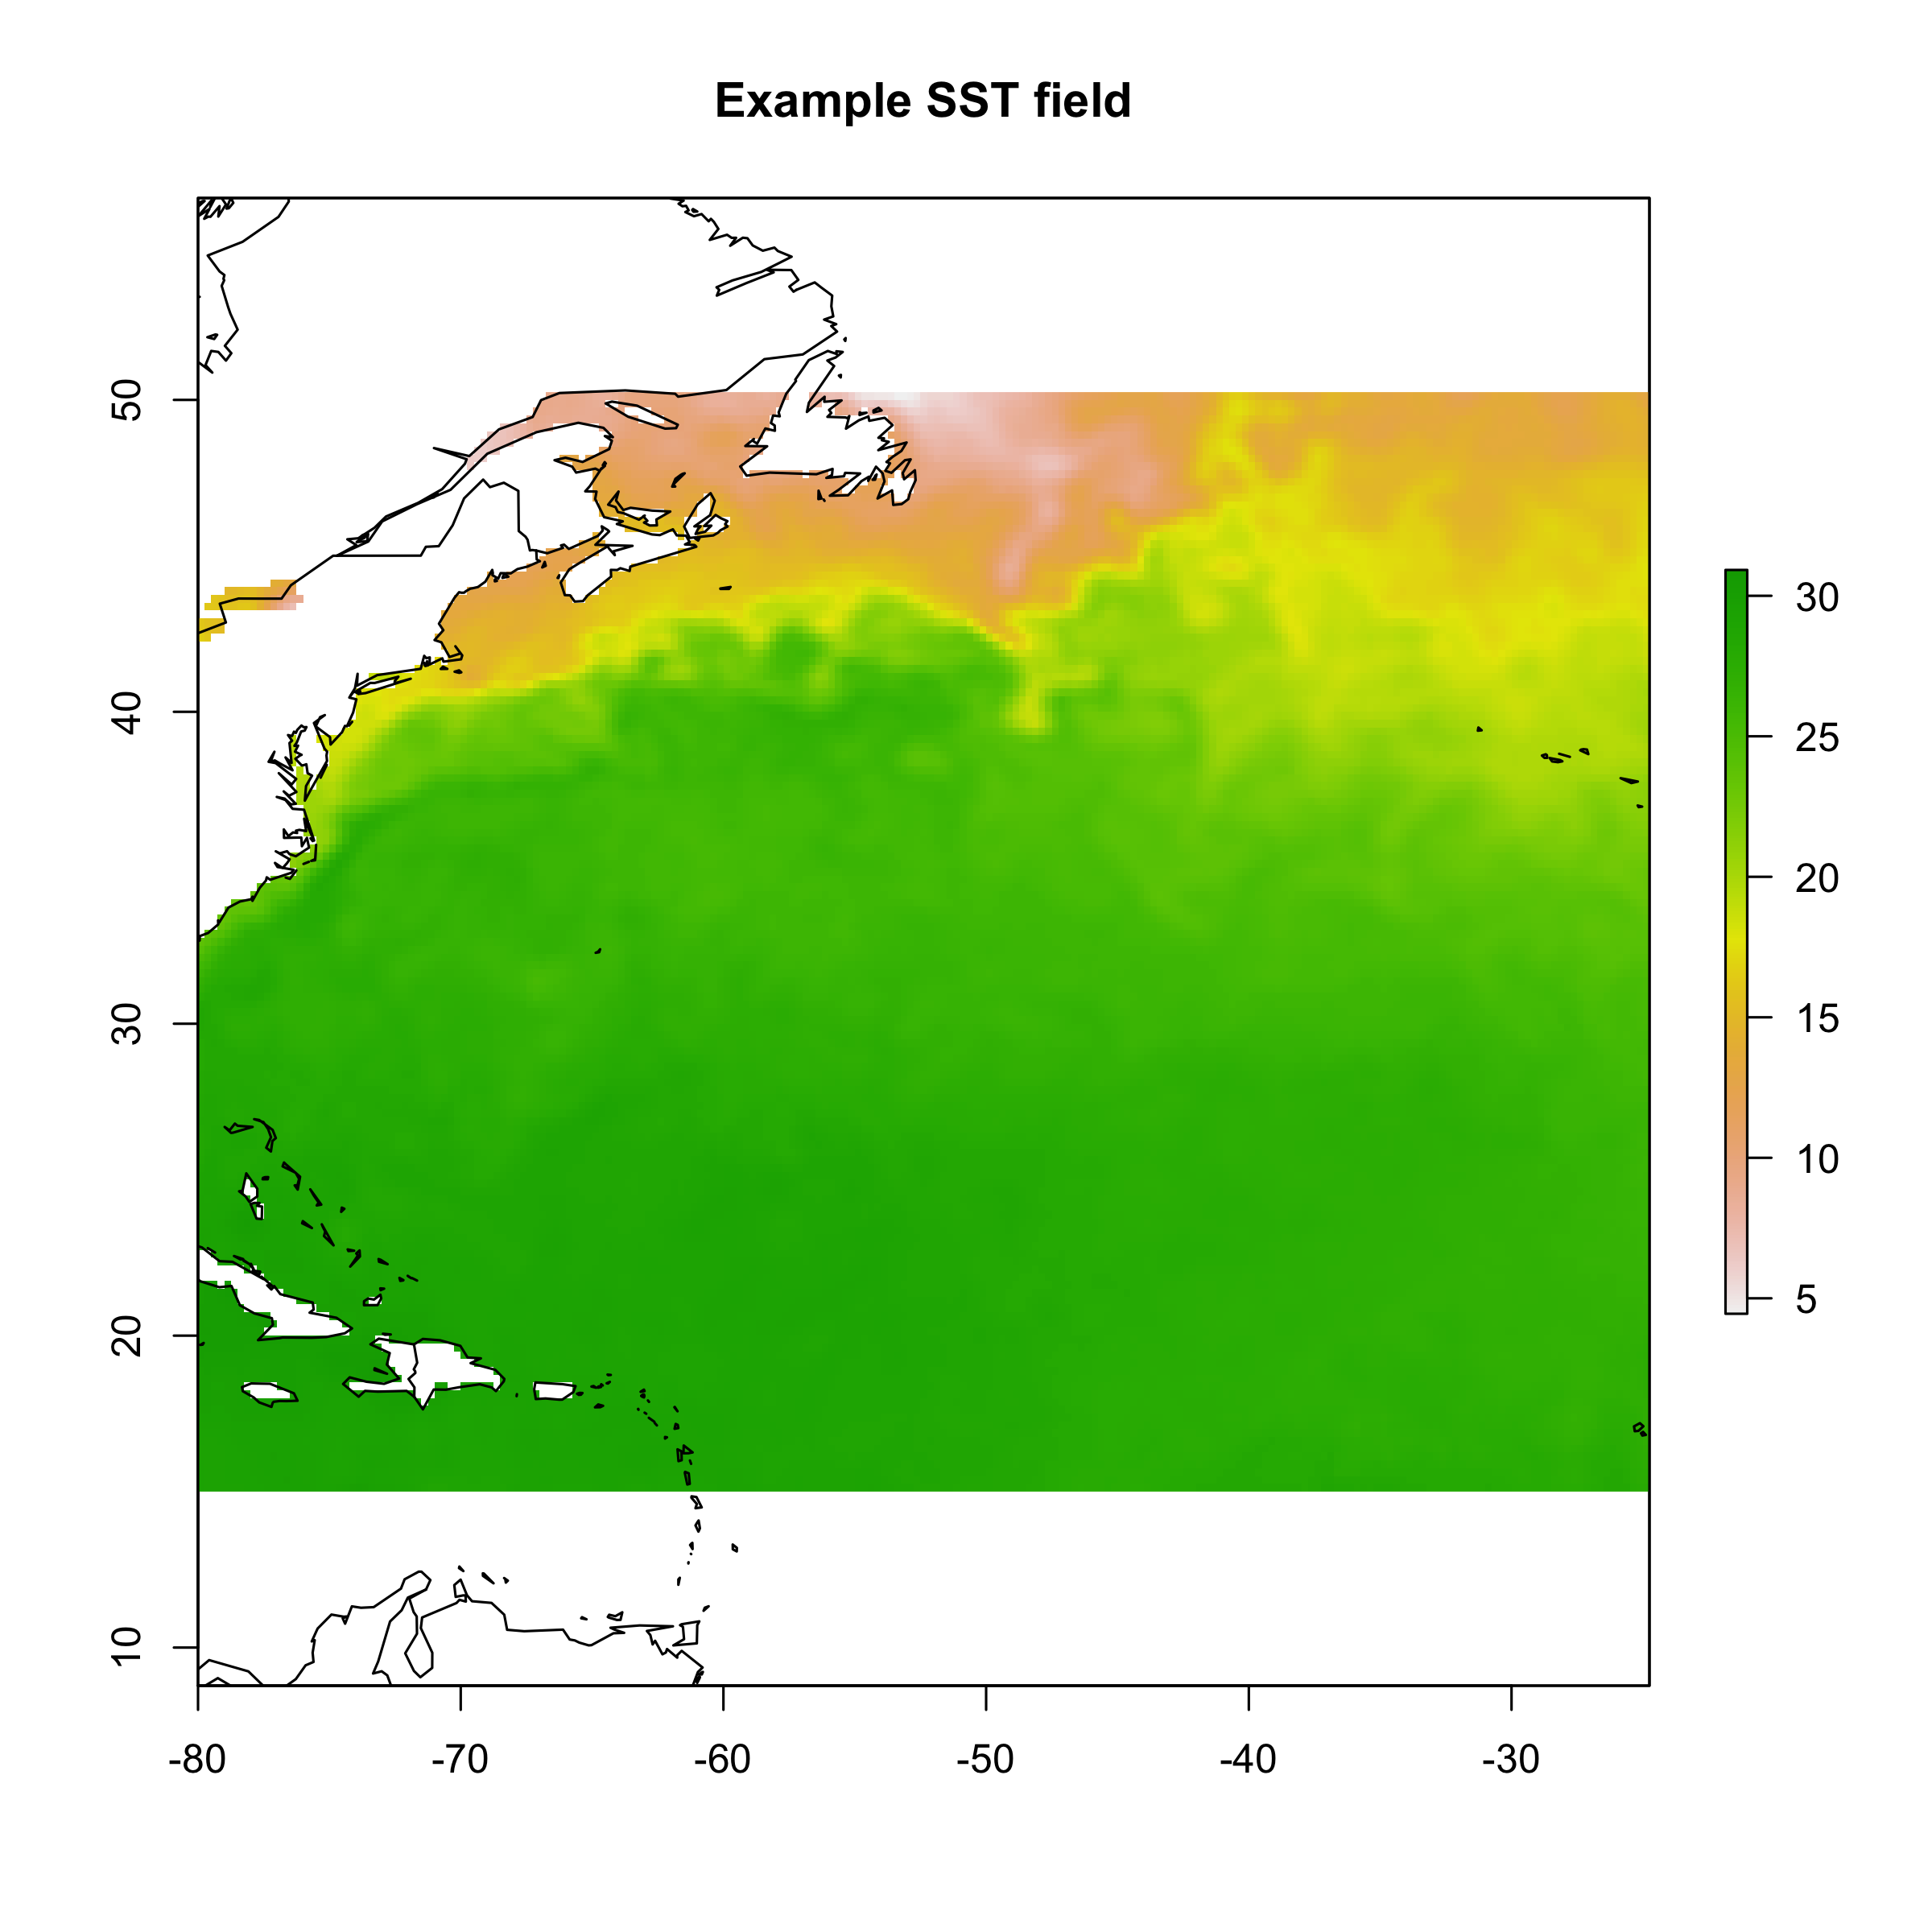
\includegraphics[width=5in, keepaspectratio]{./example_sst.png}

\subsubsection{Depth-temperature data}

As with SST above, there are a number of ways to represent temperature of the 3D ocean. While observations are nice, they are typically too sparse to generate a reliable grid on which we can calculate likelihoods. Thus, our only good option (usually) is to use oceanographic models. Data-assimilating models constantly "nudge" the model outputs to match reality and \texttt{HMMoce} includes functionality for accessing outputs of the HYbrid Coordinate Ocean Model (HYCOM). For most applications, models such as HYCOM are more likely to generate realistic likelihood results when comparing \textit{in situ} tag data to a dynamic ocean. In principle, any representation of the 3D ocean can be used for likelihood construction as is done here with HYCOM.

\begin{knitrout}\small
\definecolor{shadecolor}{rgb}{0.969, 0.969, 0.969}\color{fgcolor}\begin{kframe}
\begin{alltt}
\hlcom{## you need some representation of environmental depth-temperature in this}
\hlcom{## case we're using hycom}

\hlstd{dir} \hlkwb{<-} \hlkwd{getwd}\hlstd{()}
\hlstd{hycom.dir} \hlkwb{<-} \hlkwd{paste0}\hlstd{(dir,} \hlstr{"/EnvData/hycom/"}\hlstd{)}
\hlkwa{if} \hlstd{(}\hlopt{!}\hlkwd{dir.exists}\hlstd{(hycom.dir))} \hlkwd{dir.create}\hlstd{(hycom.dir,} \hlkwc{recursive} \hlstd{=} \hlnum{TRUE}\hlstd{)}
\hlkwa{if} \hlstd{(}\hlopt{!}\hlkwd{file.exists}\hlstd{(}\hlkwd{paste0}\hlstd{(hycom.dir,} \hlstr{"hycom_"}\hlstd{, udates[}\hlnum{1}\hlstd{],} \hlstr{".nc"}\hlstd{)))} \hlkwd{get.env}\hlstd{(udates[}\hlnum{1}\hlstd{],}
    \hlkwc{filename} \hlstd{=} \hlstr{"hycom"}\hlstd{,} \hlkwc{type} \hlstd{=} \hlstr{"hycom"}\hlstd{,} \hlkwc{spatLim} \hlstd{= sp.lim_small,} \hlkwc{save.dir} \hlstd{= hycom.dir)}

\hlstd{b} \hlkwb{<-} \hlstd{raster}\hlopt{::}\hlkwd{brick}\hlstd{(}\hlkwd{paste0}\hlstd{(hycom.dir,} \hlstr{"hycom_"}\hlstd{, udates[}\hlnum{1}\hlstd{],} \hlstr{".nc"}\hlstd{))}

\hlcom{## plot top 3 depth levels from HYCOM par(mfrow=c(3,1))}
\hlkwa{for} \hlstd{(i} \hlkwa{in} \hlkwd{c}\hlstd{(}\hlnum{1}\hlstd{,} \hlnum{10}\hlstd{,} \hlnum{20}\hlstd{)) \{}
    \hlkwd{plot}\hlstd{(b[[i]])}
    \hlkwd{world}\hlstd{(}\hlkwc{add} \hlstd{= T)}
\hlstd{\}}
\end{alltt}
\end{kframe}
\end{knitrout}

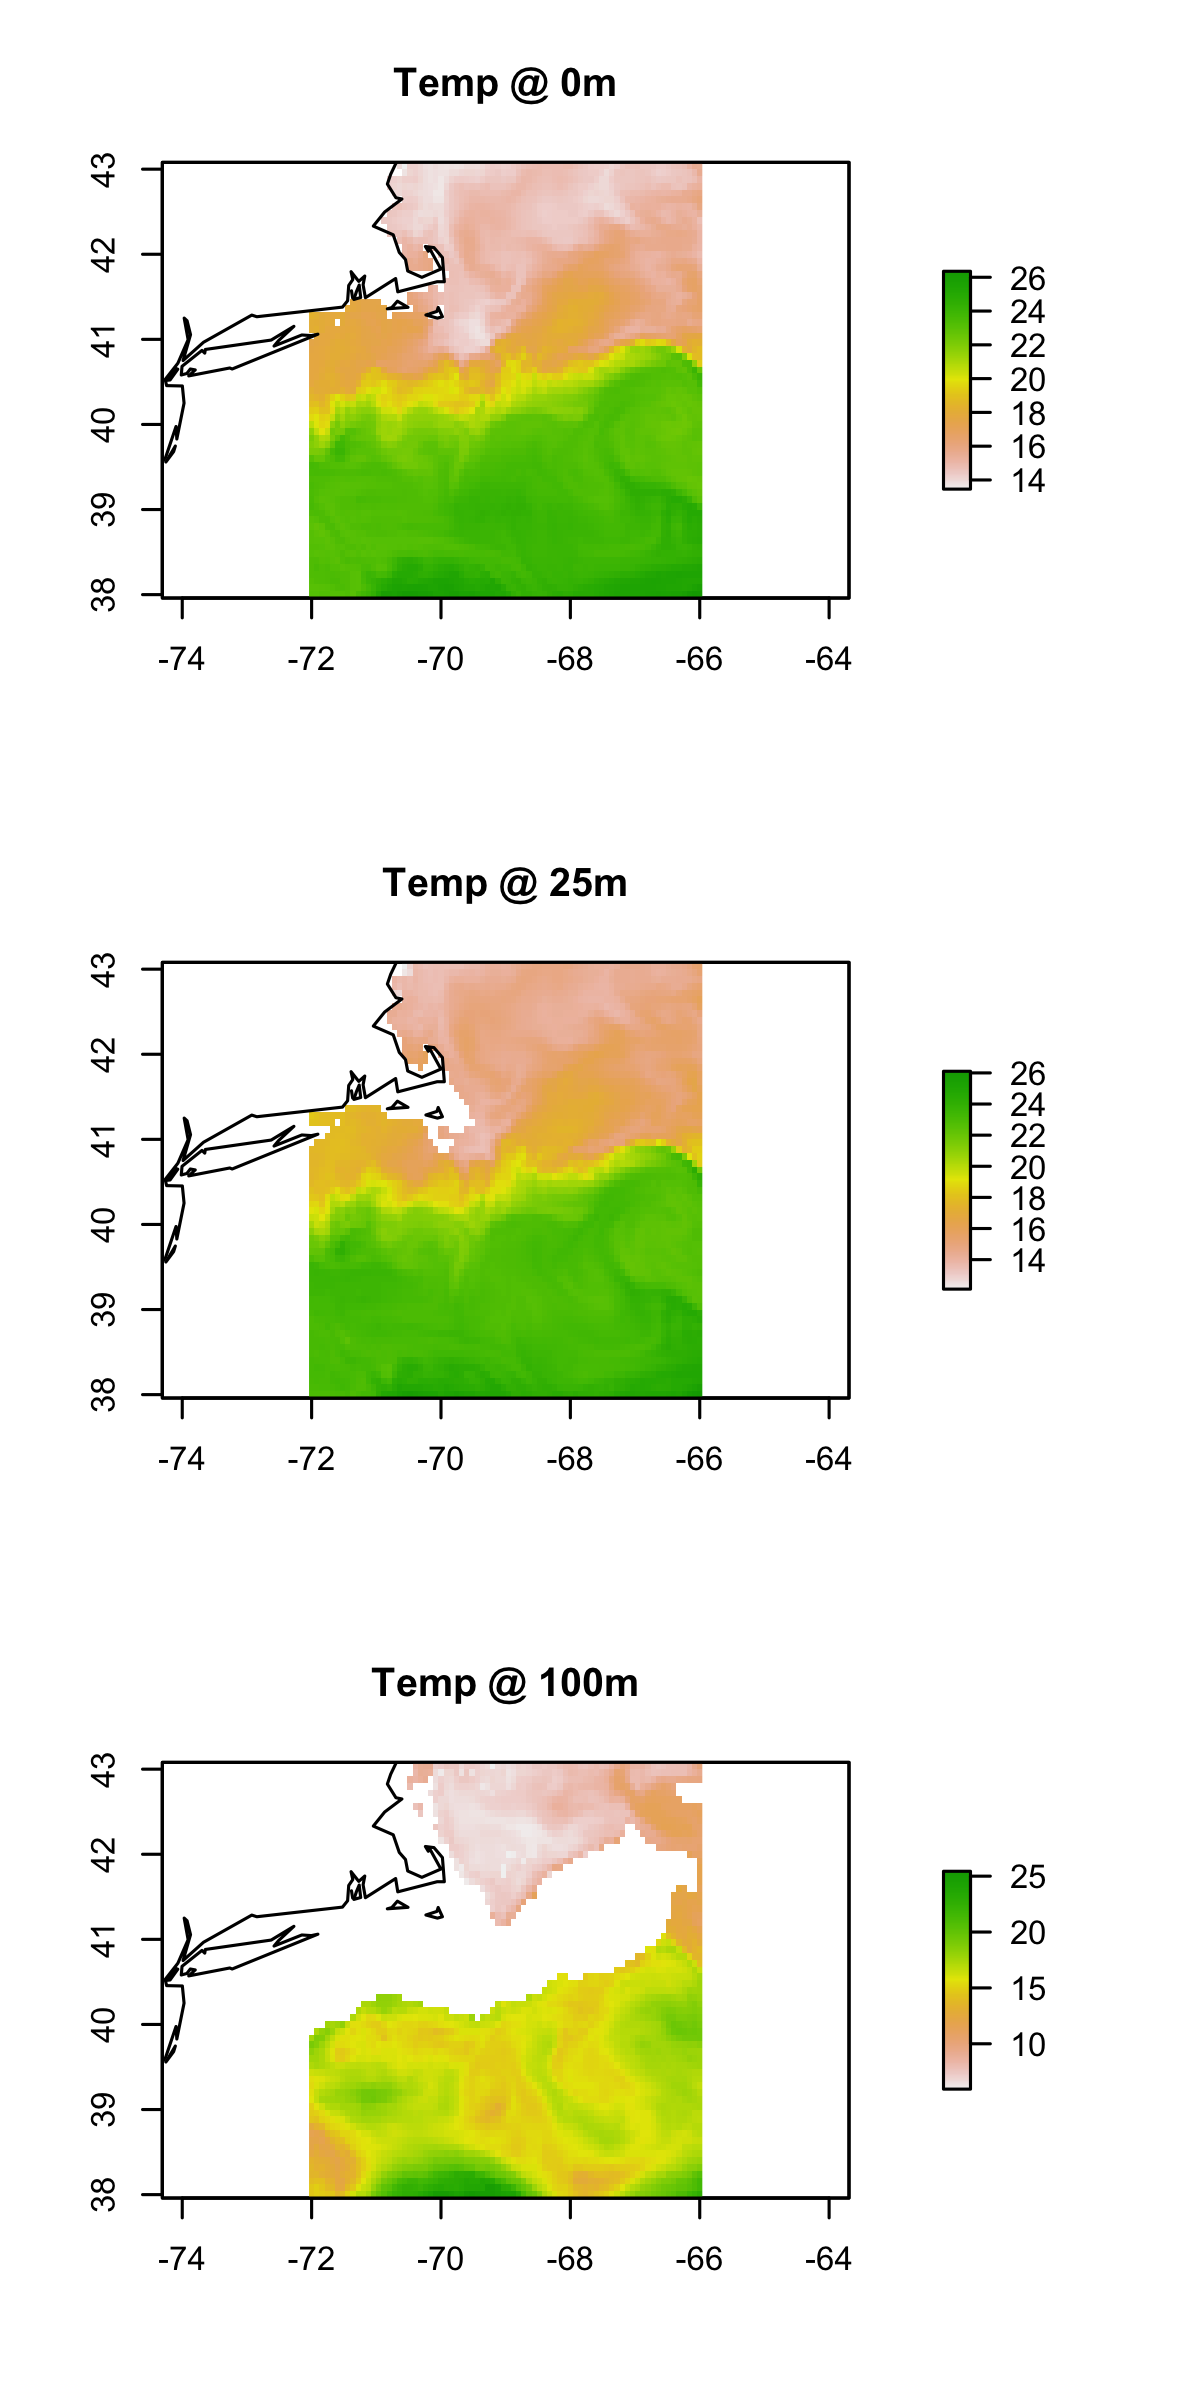
\includegraphics[width=5in, keepaspectratio]{./example_hycom.png}

\subsubsection{Bathymetry}

The last "environmental" dataset we need is bathymetry. Bathymetry has multiple uses in \texttt{HMMoce} but is primarily used as a mask that eliminates portions of a likelihood grid that are shallower than the maximum depth the tag recorded during a given timestep (\ie the likelihood has to incorporate bottom depth at least as deep as the animal's tag recorded). For primarily benthic species, bathymetry can also be used to generate a likelihood based on the tag-recorded depth compared to bottom depth.

\begin{knitrout}\small
\definecolor{shadecolor}{rgb}{0.969, 0.969, 0.969}\color{fgcolor}\begin{kframe}
\begin{alltt}
\hlstd{bathy.dir} \hlkwb{<-} \hlkwd{paste0}\hlstd{(dir,} \hlstr{"/EnvData/bathy/"}\hlstd{)}
\hlkwa{if} \hlstd{(}\hlopt{!}\hlkwd{dir.exists}\hlstd{(bathy.dir))} \hlkwd{dir.create}\hlstd{(bathy.dir,} \hlkwc{recursive} \hlstd{=} \hlnum{TRUE}\hlstd{)}

\hlkwa{if} \hlstd{(}\hlopt{!}\hlkwd{file.exists}\hlstd{(}\hlkwd{paste0}\hlstd{(bathy.dir,} \hlstr{"bathy.nc"}\hlstd{))) \{}
    \hlstd{bathy} \hlkwb{<-} \hlstd{HMMoce}\hlopt{::}\hlkwd{get.bath.data}\hlstd{(sp.lim_small}\hlopt{$}\hlstd{lonmin, sp.lim_small}\hlopt{$}\hlstd{lonmax,}
        \hlstd{sp.lim_small}\hlopt{$}\hlstd{latmin, sp.lim_small}\hlopt{$}\hlstd{latmax,} \hlkwc{folder} \hlstd{= bathy.dir,} \hlkwc{res} \hlstd{=} \hlnum{1}\hlstd{)}
\hlstd{\}} \hlkwa{else} \hlstd{\{}
    \hlcom{## OR (once downloaded and reading the .nc later)}
    \hlstd{bathy} \hlkwb{<-} \hlkwd{irregular_ncToRaster}\hlstd{(}\hlkwd{paste0}\hlstd{(bathy.dir,} \hlstr{"bathy.nc"}\hlstd{),} \hlkwc{varid} \hlstd{=} \hlstr{"topo"}\hlstd{)}
\hlstd{\}}

\hlcom{## example bathymetry data}
\hlkwd{plot}\hlstd{(bathy,} \hlkwc{main} \hlstd{=} \hlstr{"Example bathymetry field"}\hlstd{)}
\hlkwd{world}\hlstd{(}\hlkwc{add} \hlstd{= T)}
\end{alltt}
\end{kframe}
\end{knitrout}

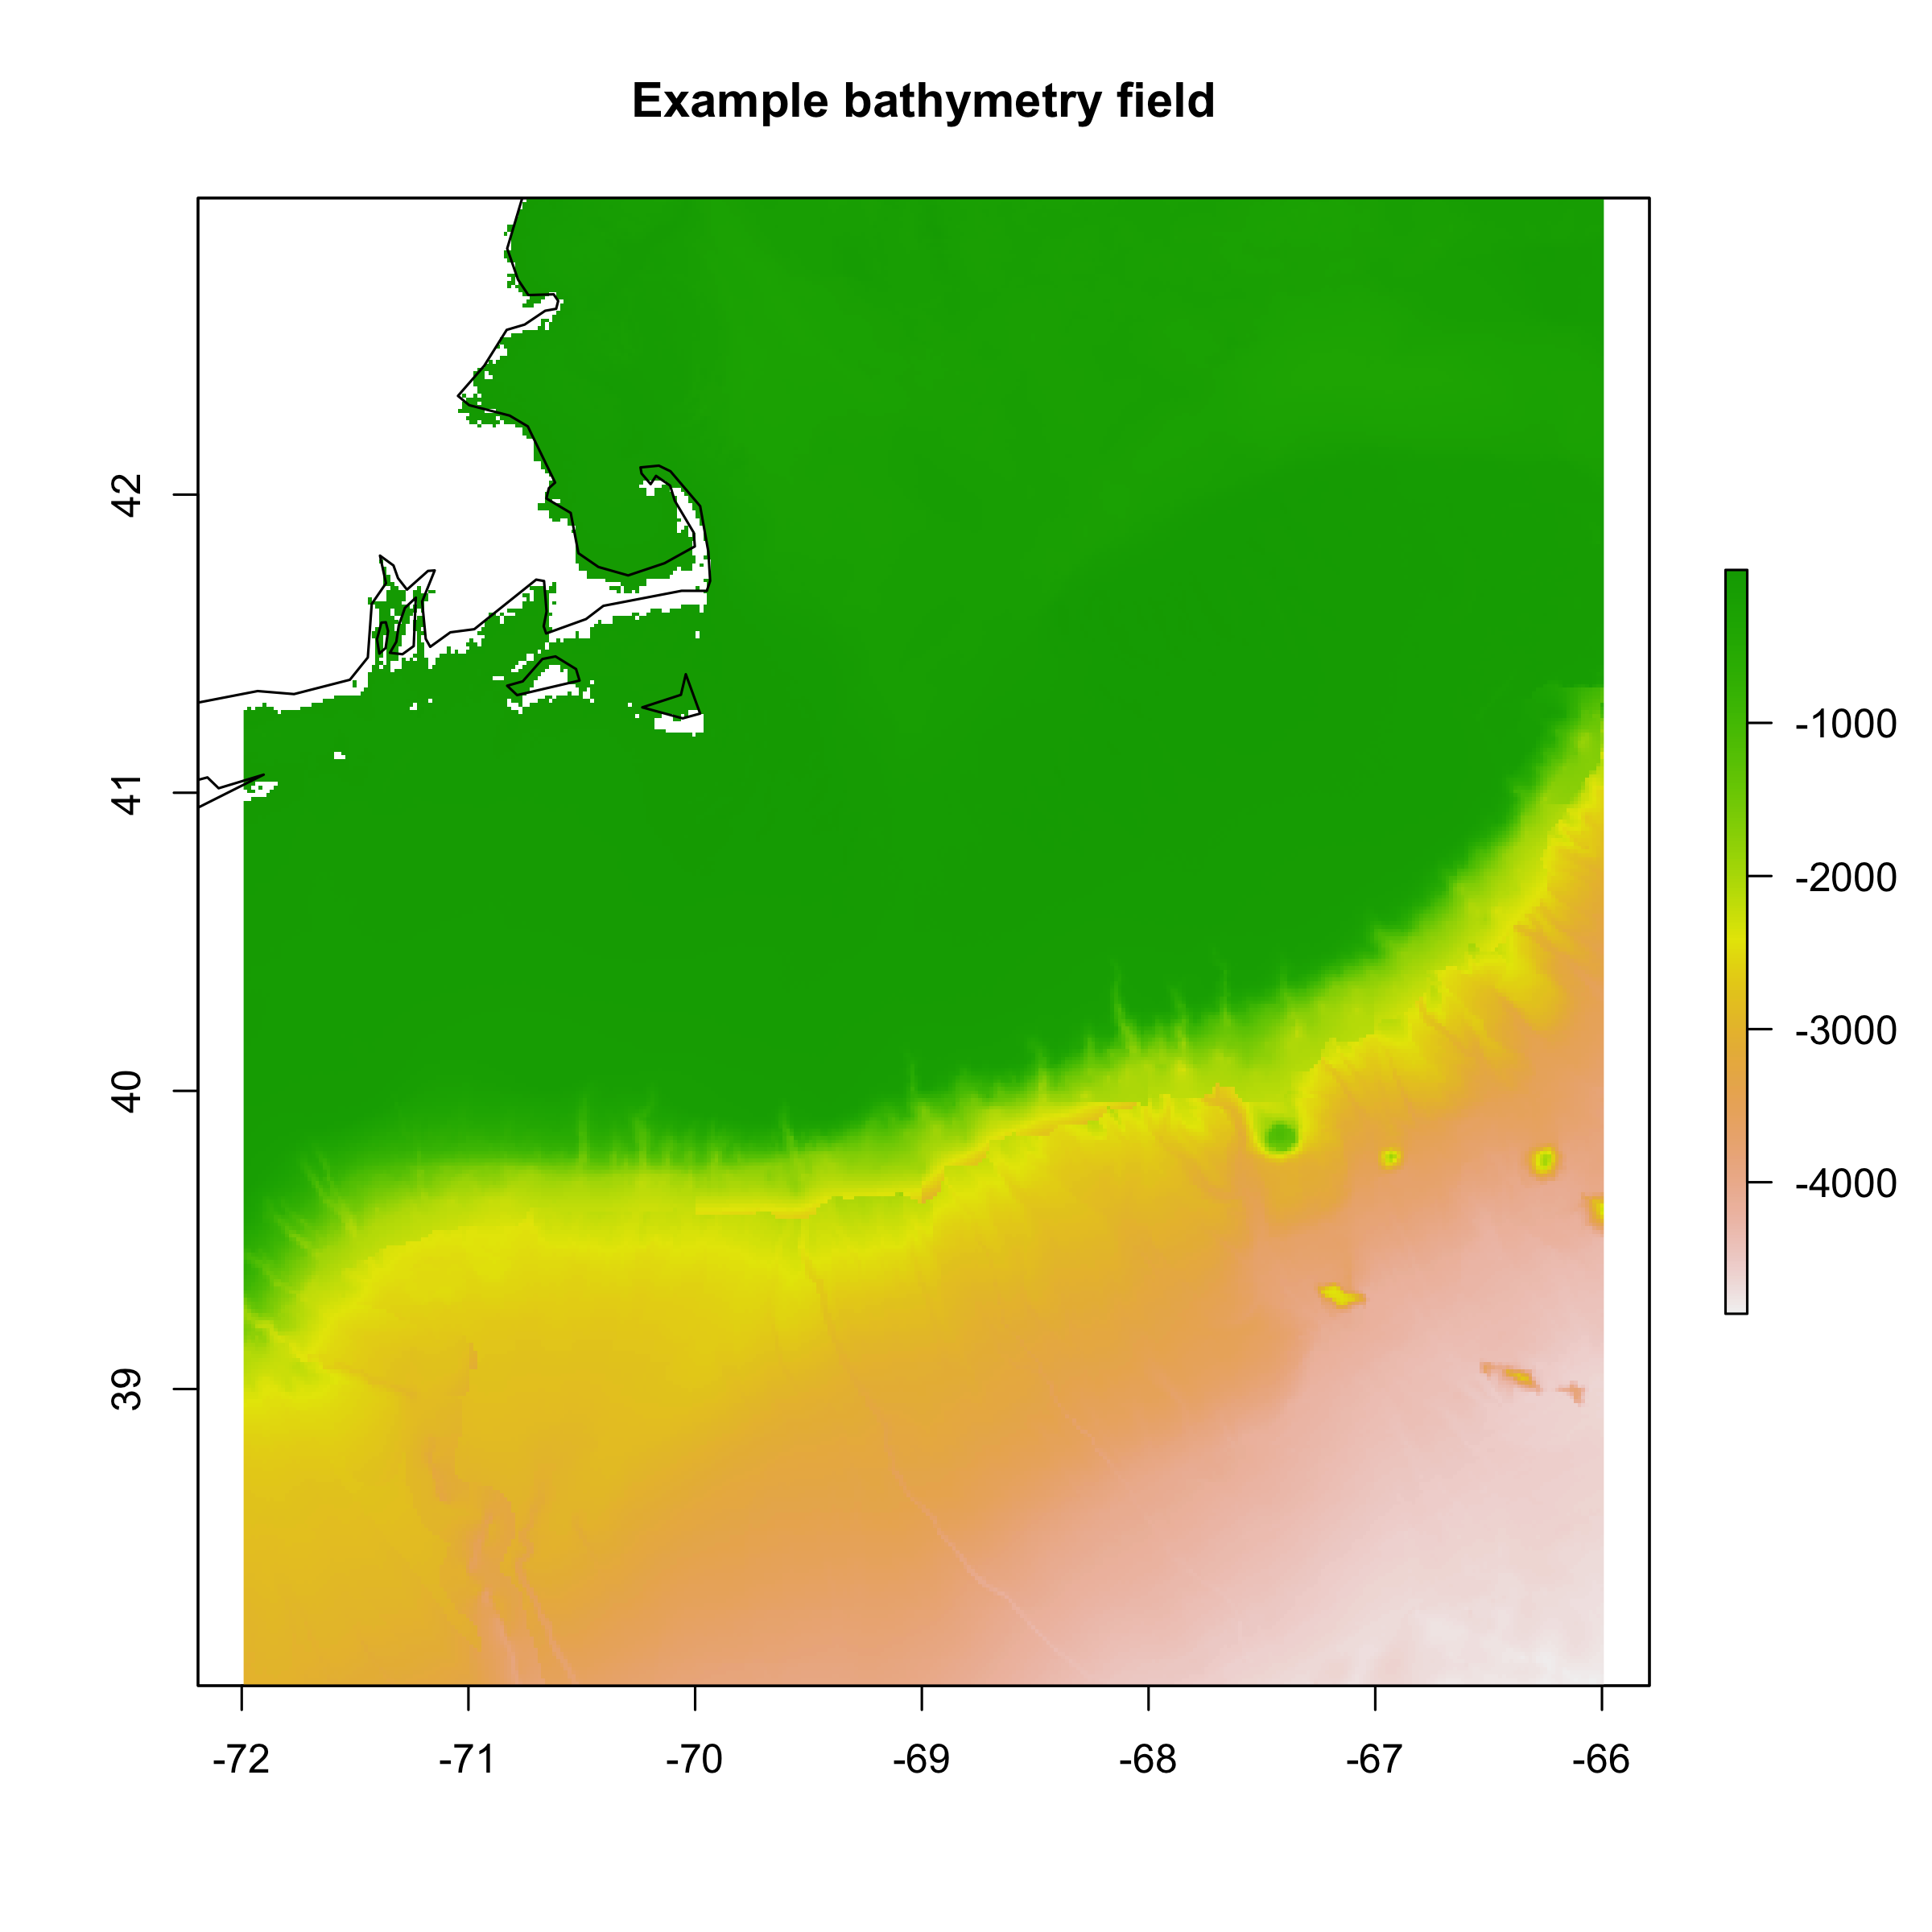
\includegraphics[width=5in, keepaspectratio]{./example_bathy.png}

\subsection{Observation likelihoods} \label{sec:lik}

The basic premise of the observation likelihoods is that we compare a tag-based data stream to some representation of the environment to generate a likelihood surface. This comparison generates information about the likely location of the animal in the global ocean. Light levels and SST are the current paradigm for fish tracking and are the most straightforward to use for positioning. Three-dimensional depth-temperature data are more complex and computationally intensive but can provide rich information about oceanographic characteristics and water masses that animals experience as they move \citep[\eg][]{Braun2018b}. Each data type has its own likelihood function(s) that does the grunt work for you. It often makes sense to build all the appropriate likelihoods given your tag data and study species and use model selection to determine the "best" combination of likelihoods \citep[for example, see][and section \ref{sec:multiple}]{Braun2018a}.

\subsubsection{Light likelihood}

Light-based geolocation is a complicated topic with a myriad of potential implementations for generating light-based likelihoods. For now, \texttt{HMMoce} has two main treatments of light to inform geolocation estimates (Sec. \ref{sec:light-data}). The simplest is using tag-based light levels to estimate sunrise and sunset times and thus position (\texttt{calc.srss}). This is usually an overly simplistic treatment of this data so we often 1) throw out latitude estimates and only keep longitude and 2) get a lot of bad location information, particularly from species that don't frequent the photic zone. For example, a surface-oriented species that dives below the photic zone 30 minutes before sunset would generate an artificial sunset time 30 minutes early, causing $\sim$8$^\circ$ longitudinal difference in position estimate! The other approach currently implemented in \texttt{HMMoce} generates likelihoods based on existing light-based position estimates(\texttt{calc.lightloc}). Most manufacturers either provide the analysis or the analysis software to generate light-based position estimates. For example, Wildlife Computers uses a thresholding algorithm (hill ref) in their GPE2 software that allows user-controlled QC of light curves in a GUI. While this software has been replaced by their cloud-based GPE3 algorithm, GPE2 remains the tool of choice for this specific analysis as the user retains some control over the conversion of light curves to location estimates and the ability to visually check the quality of these curves. Other manufacturers generate similar light-based position outputs such as Lotek's daily summary for archival tags. Additional light-based options will be implemented in the future as they become available and proven for marine animal telemetry. To that end, we are happy to receive feedback via Github on methods to include or simply submit a pull request.

\begin{knitrout}\small
\definecolor{shadecolor}{rgb}{0.969, 0.969, 0.969}\color{fgcolor}\begin{kframe}
\begin{alltt}
\hlcom{# LIGHT-BASED LIKELIHOODS}
\hlstd{L.light.srss} \hlkwb{<-} \hlkwd{calc.srss}\hlstd{(light,} \hlkwc{locs.grid} \hlstd{= locs.grid,} \hlkwc{dateVec} \hlstd{= dateVec,} \hlkwc{res} \hlstd{=} \hlnum{1}\hlstd{,}
    \hlkwc{focalDim} \hlstd{=} \hlnum{15}\hlstd{)}
\hlstd{L.light} \hlkwb{<-} \hlkwd{calc.lightloc}\hlstd{(lightloc,} \hlkwc{locs.grid} \hlstd{= locs.grid,} \hlkwc{dateVec} \hlstd{= dateVec,}
    \hlkwc{errEll} \hlstd{=} \hlnum{TRUE}\hlstd{)}
\end{alltt}
\end{kframe}
\end{knitrout}


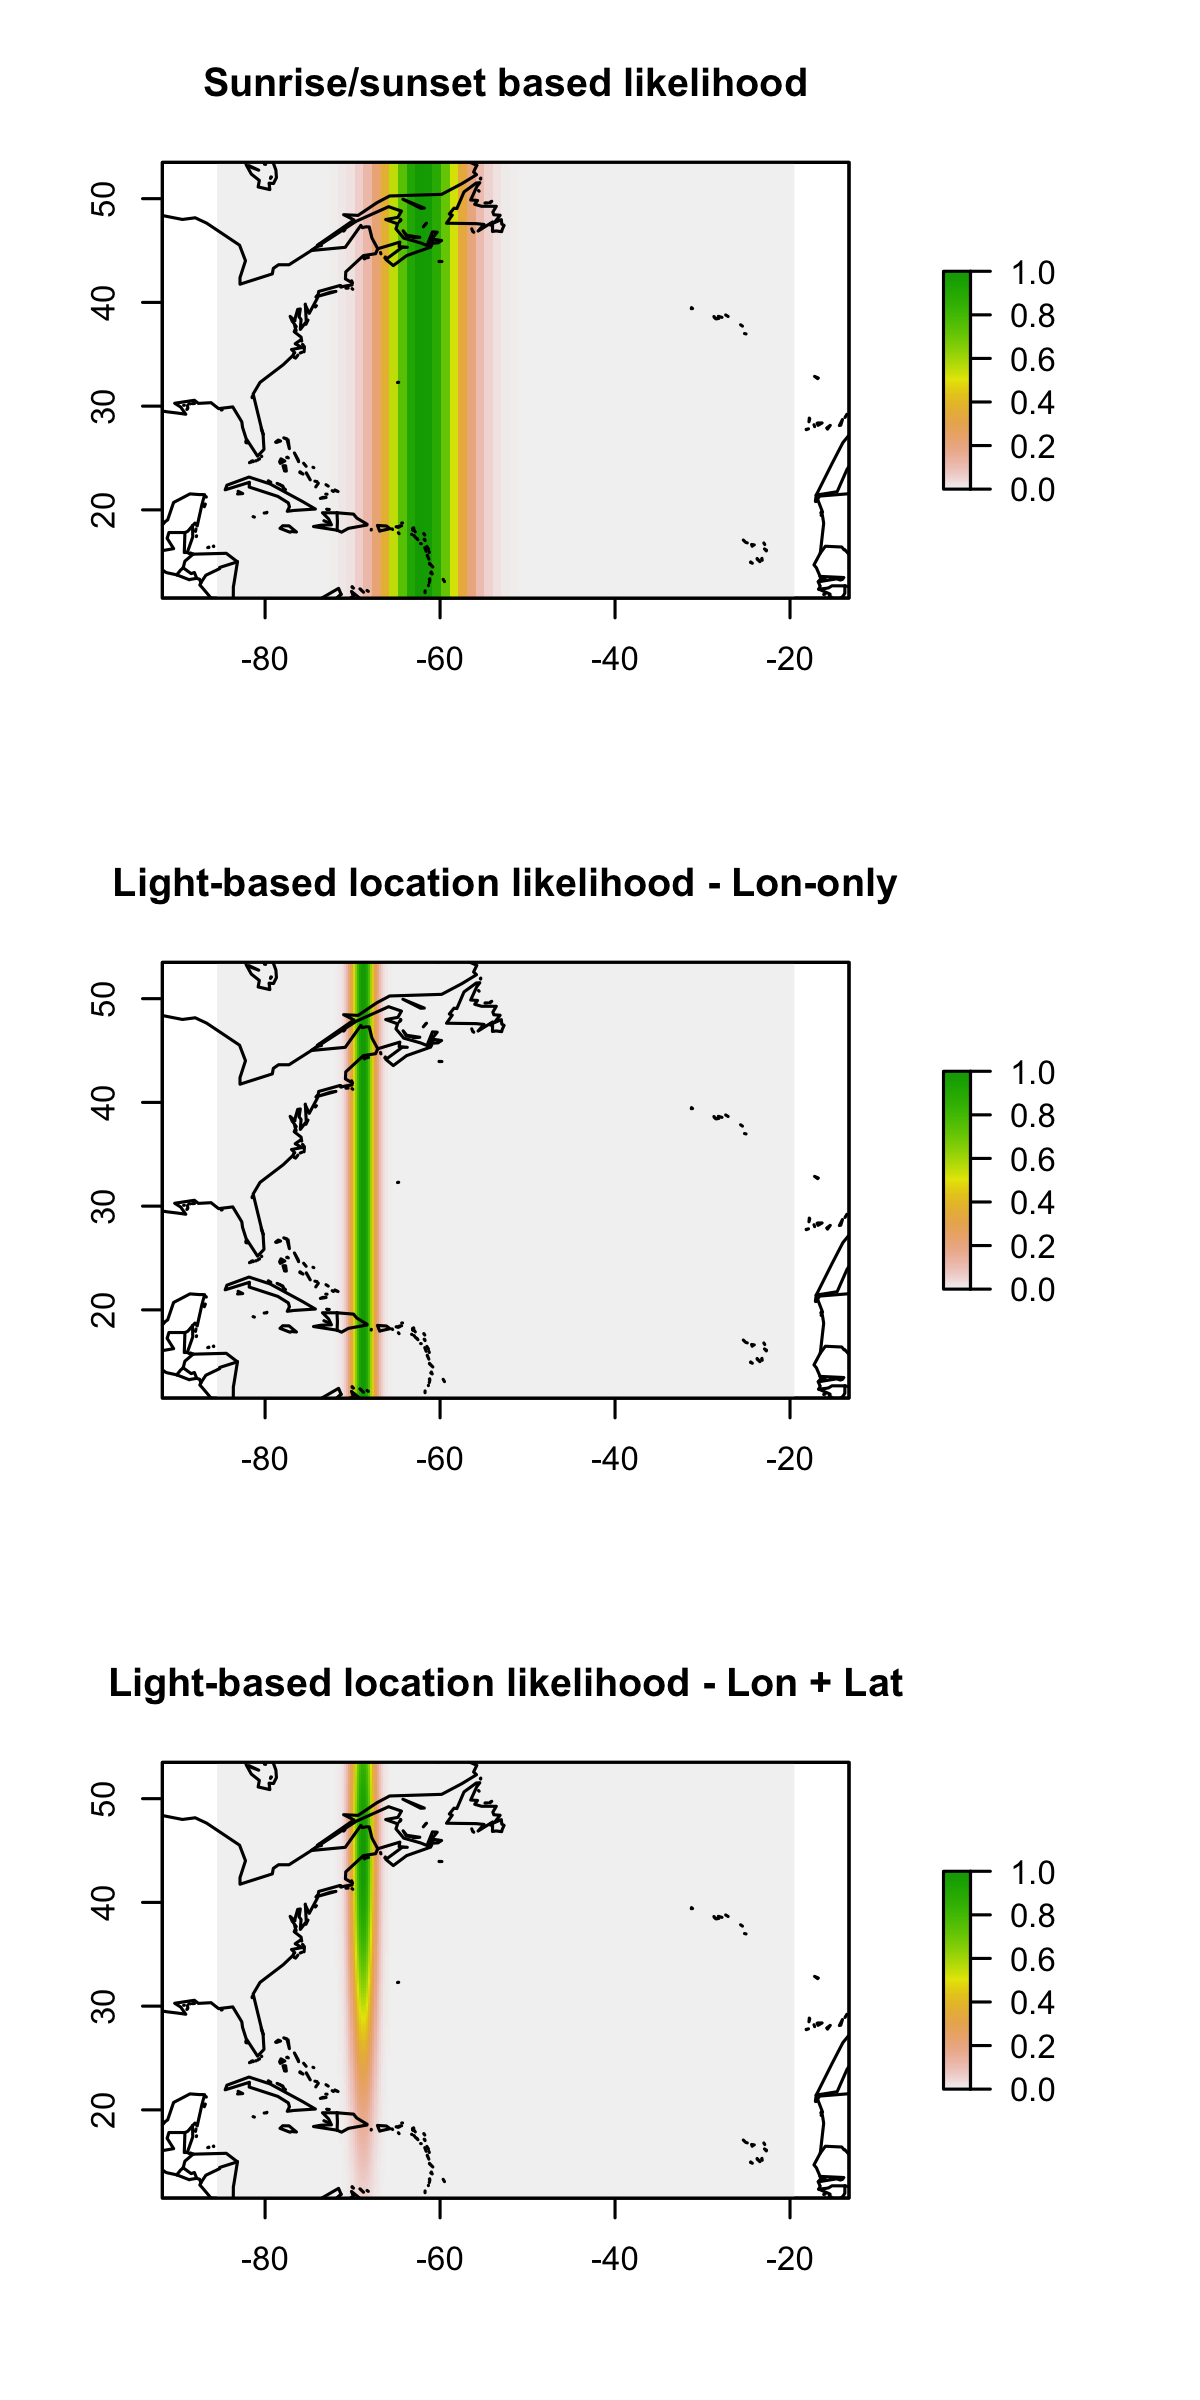
\includegraphics[width=5in, keepaspectratio]{./example_light_lik.png}

\subsubsection{SST likelihood}

SST-based likelihoods are perhaps among the most simple, and often informative, for geolocation as SST can be highly dynamic and exhibit strong gradients over relatively small spatial scales. If your study animal regularly visits the surface and thus collects SST data, it's likely that including that information will improve your geolocation results. In \texttt{HMMoce}, tag-based SST data is represented as a daily range in SST $\pm$ error (currently defaults to 1\%) and that SST envelope is then compared to a remotely-sensed SST product to generate a likelihood surface.

\begin{knitrout}\small
\definecolor{shadecolor}{rgb}{0.969, 0.969, 0.969}\color{fgcolor}\begin{kframe}
\begin{alltt}
\hlcom{# SST LIKELIHOODS}
\hlstd{L.sst} \hlkwb{<-} \hlkwd{calc.sst}\hlstd{(tag.sst,} \hlkwc{filename} \hlstd{=} \hlstr{"oisst"}\hlstd{,} \hlkwc{sst.dir} \hlstd{= sst.dir,} \hlkwc{dateVec} \hlstd{= dateVec,}
    \hlkwc{sens.err} \hlstd{=} \hlnum{1}\hlstd{)}

\hlcom{## identical to above but in parallel}
\hlstd{L.sst} \hlkwb{<-} \hlkwd{calc.sst.par}\hlstd{(tag.sst,} \hlkwc{filename} \hlstd{=} \hlstr{"oisst"}\hlstd{,} \hlkwc{sst.dir} \hlstd{= sst.dir,} \hlkwc{dateVec} \hlstd{= dateVec,}
    \hlkwc{sens.err} \hlstd{=} \hlnum{1}\hlstd{,} \hlkwc{ncores} \hlstd{=} \hlnum{2}\hlstd{)}
\end{alltt}
\end{kframe}
\end{knitrout}


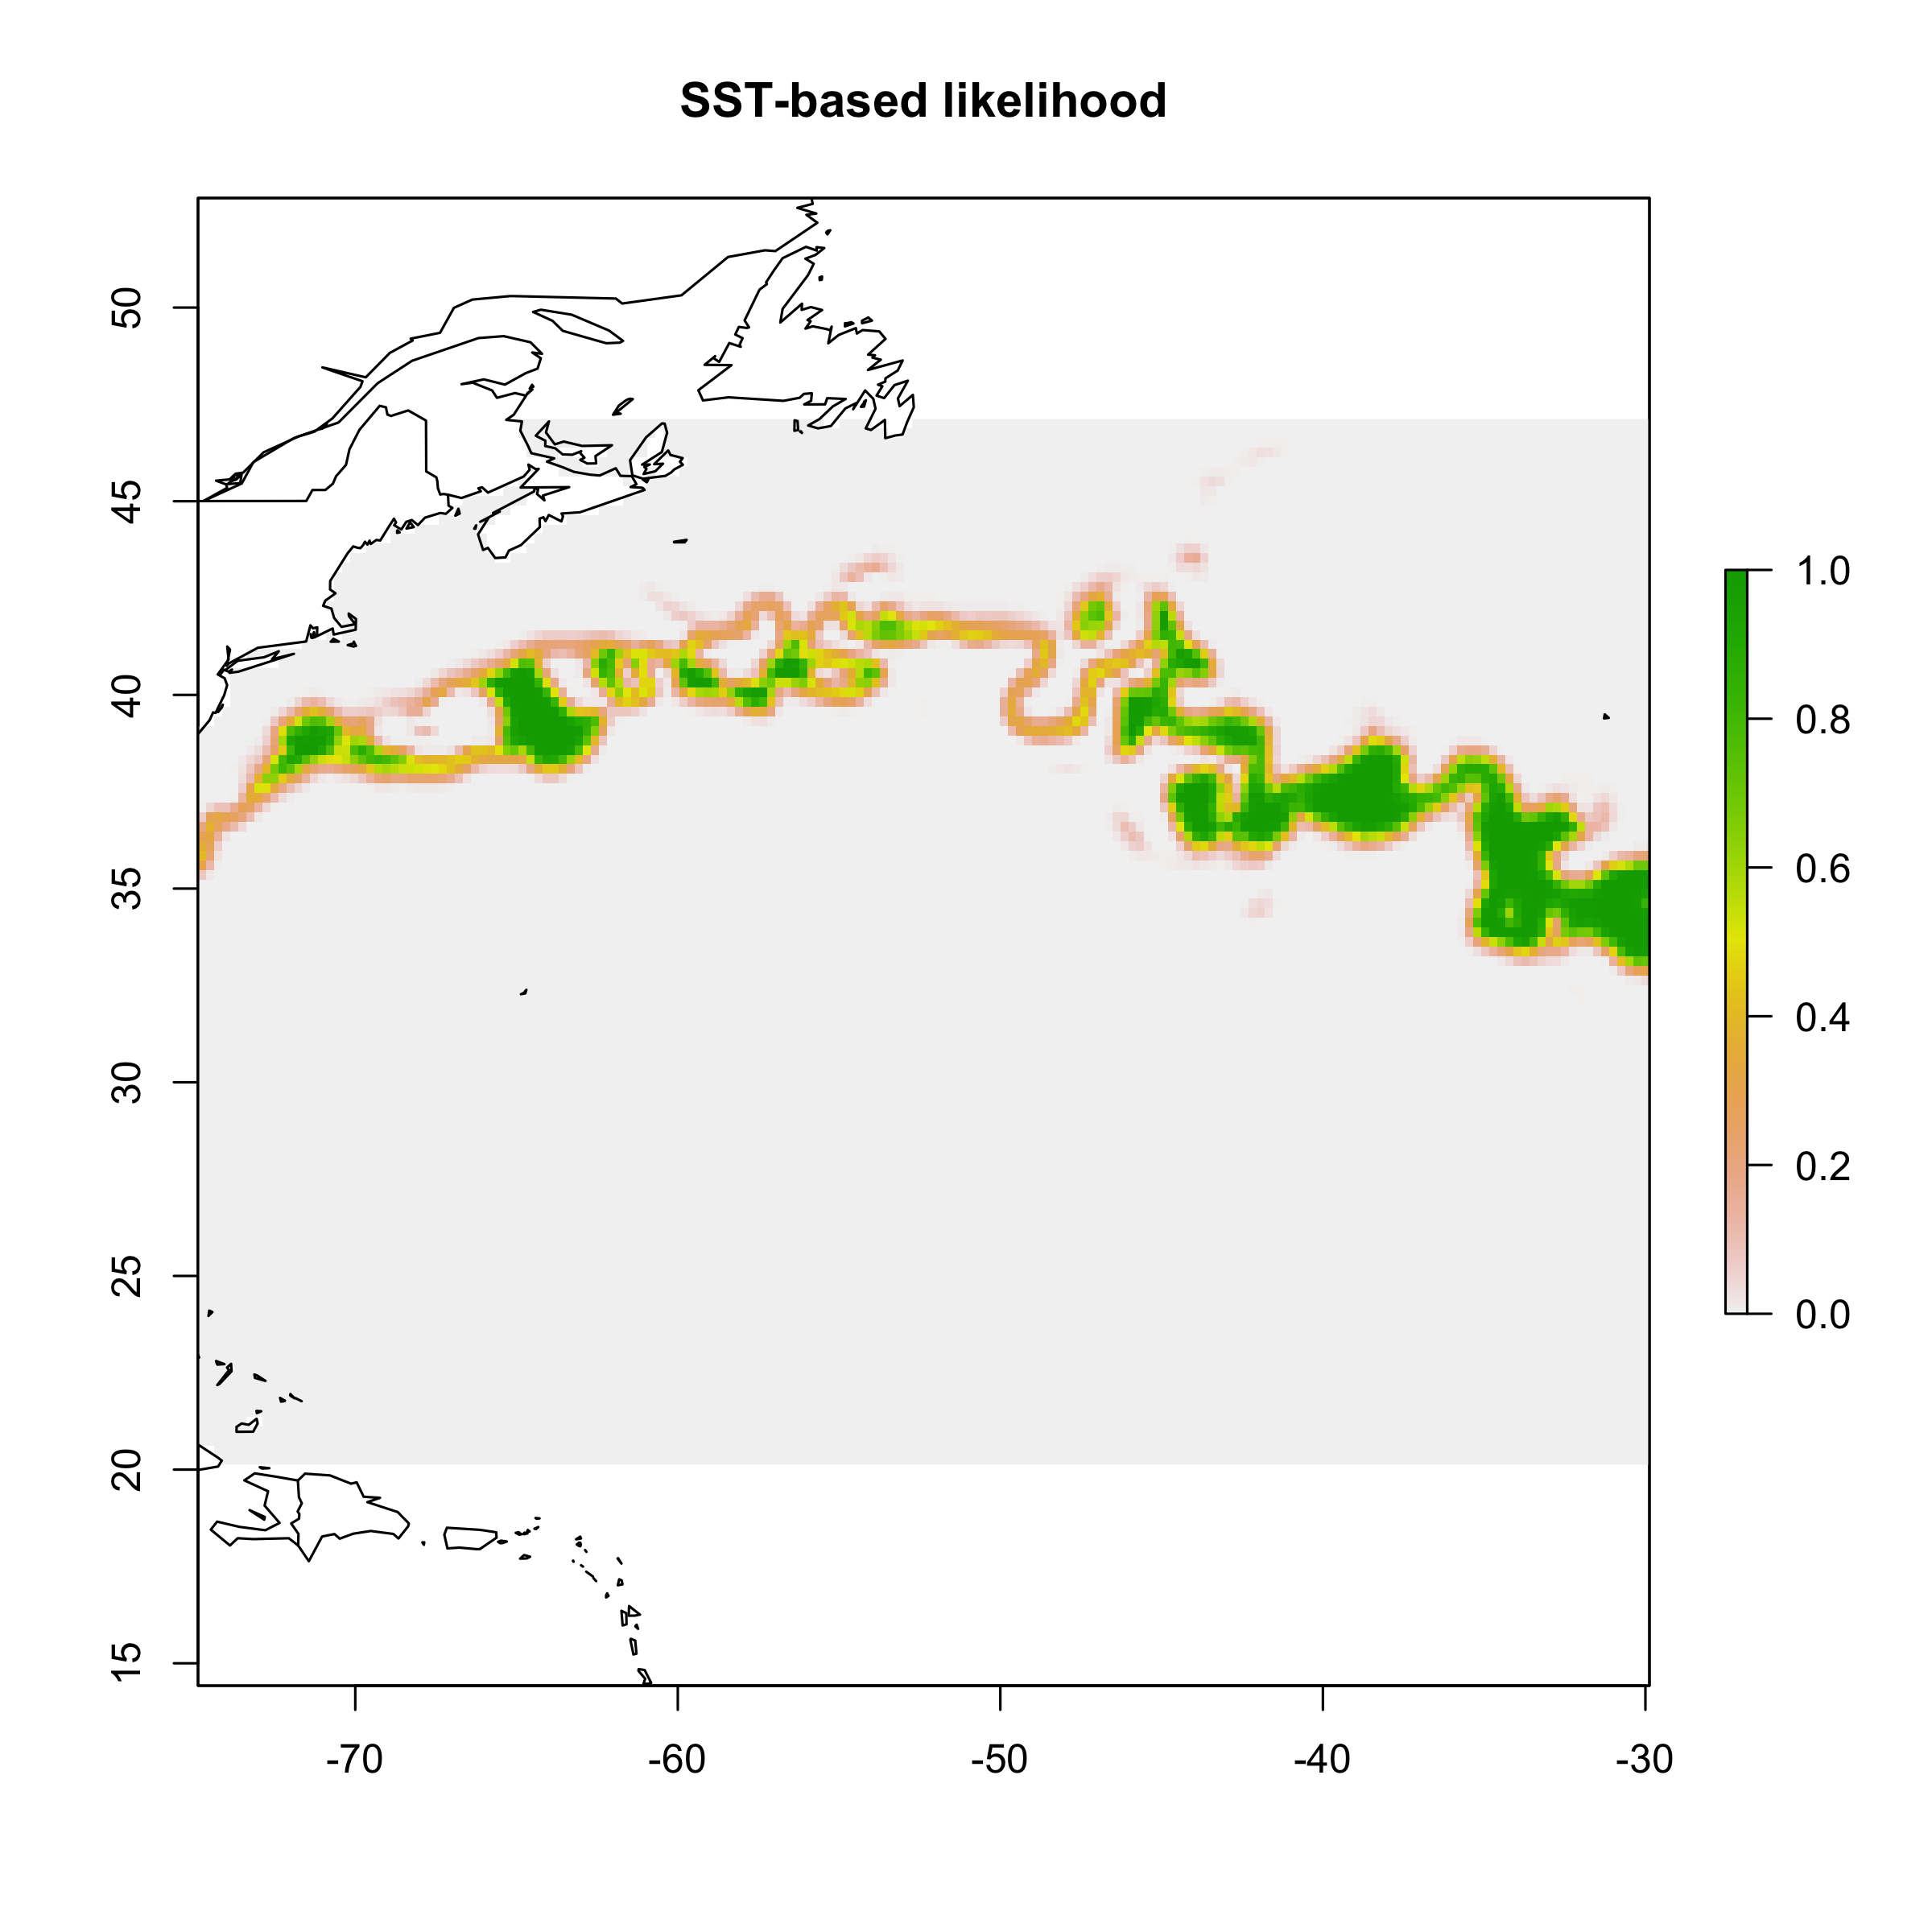
\includegraphics[width=5in, keepaspectratio]{./example_sst_lik.png}


\subsubsection{3D depth-temperature likelihood}

The depth-temperature based likelihoods allow users to generate 3D likelihoods for tagged animals to improve position estimates, which is particularly useful for study species that rarely visit the photic zone during the day \citep[(e.g. swordfish,][]{Neilson2009, Braun2019} or spend considerable periods of time in the mesopelagic \citep[e.g. basking sharks,][]{Skomal2009, Braun2018b}. In \texttt{HMMoce}, there are currently two approaches to using the 3D data for geolocation. The first follows \citep{Luo2015} by integrating profile data to calculate Ocean Heat Content (OHC). We integrate tag-based depth-temperature data from a given isotherm (default or user-selected) to the surface to calculate the "heat content" of that layer measured by the tagged animal. Similarly, we perform the same integration on the model ocean as represented in the HYbrid Coordinate Ocean Model ([HYCOM](http://hycom.org/)) and compare the two integrated metrics to generate a likelihood surface representing the animal's estimated daily position. The second approach is to use the profile in 3D space and compare it to oceanography at measured depth levels. This uses the same tag-based depth-temperature data (not integrated) and compares it to modeled oceanography (such as HYCOM). In either case, we use a linear regression to predict the tag-based temperature at the standard depth levels measured in the oceanographic datasets (this is why we generate custom depth-temperature tag data to match oceanographic depth levels whenever possible, \ref{sec:tag-data}). Then a likelihood is calculated in the same fashion by comparing temperature from the tag to ocean temperature at each depth level and resulting likelihood layers are multiplied across depth levels to result in a single daily likelihood layer based on the tagged animal's dive data. Because these can be very computationally demanding, parallelized calculation functions are available for all three depth-temperature based likelihood functions.

\begin{knitrout}\small
\definecolor{shadecolor}{rgb}{0.969, 0.969, 0.969}\color{fgcolor}\begin{kframe}
\begin{alltt}
\hlcom{# OCEAN HEAT CONTENT (INTEGRATED PDTS)}
\hlstd{L.ohc} \hlkwb{<-} \hlkwd{calc.ohc}\hlstd{(pdt,} \hlkwc{filename} \hlstd{=} \hlstr{"hycom"}\hlstd{,} \hlkwc{ohc.dir} \hlstd{= hycom.dir,} \hlkwc{dateVec} \hlstd{= dateVec,}
    \hlkwc{isotherm} \hlstd{=} \hlstr{""}\hlstd{,} \hlkwc{use.se} \hlstd{= F)}
\hlcom{## the parallel version: L.ohc <- calc.ohc.par(pdt, filename='hycom', ohc.dir}
\hlcom{## = hycom.dir, dateVec = dateVec, isotherm = '', use.se = F)}
\end{alltt}
\end{kframe}
\end{knitrout}
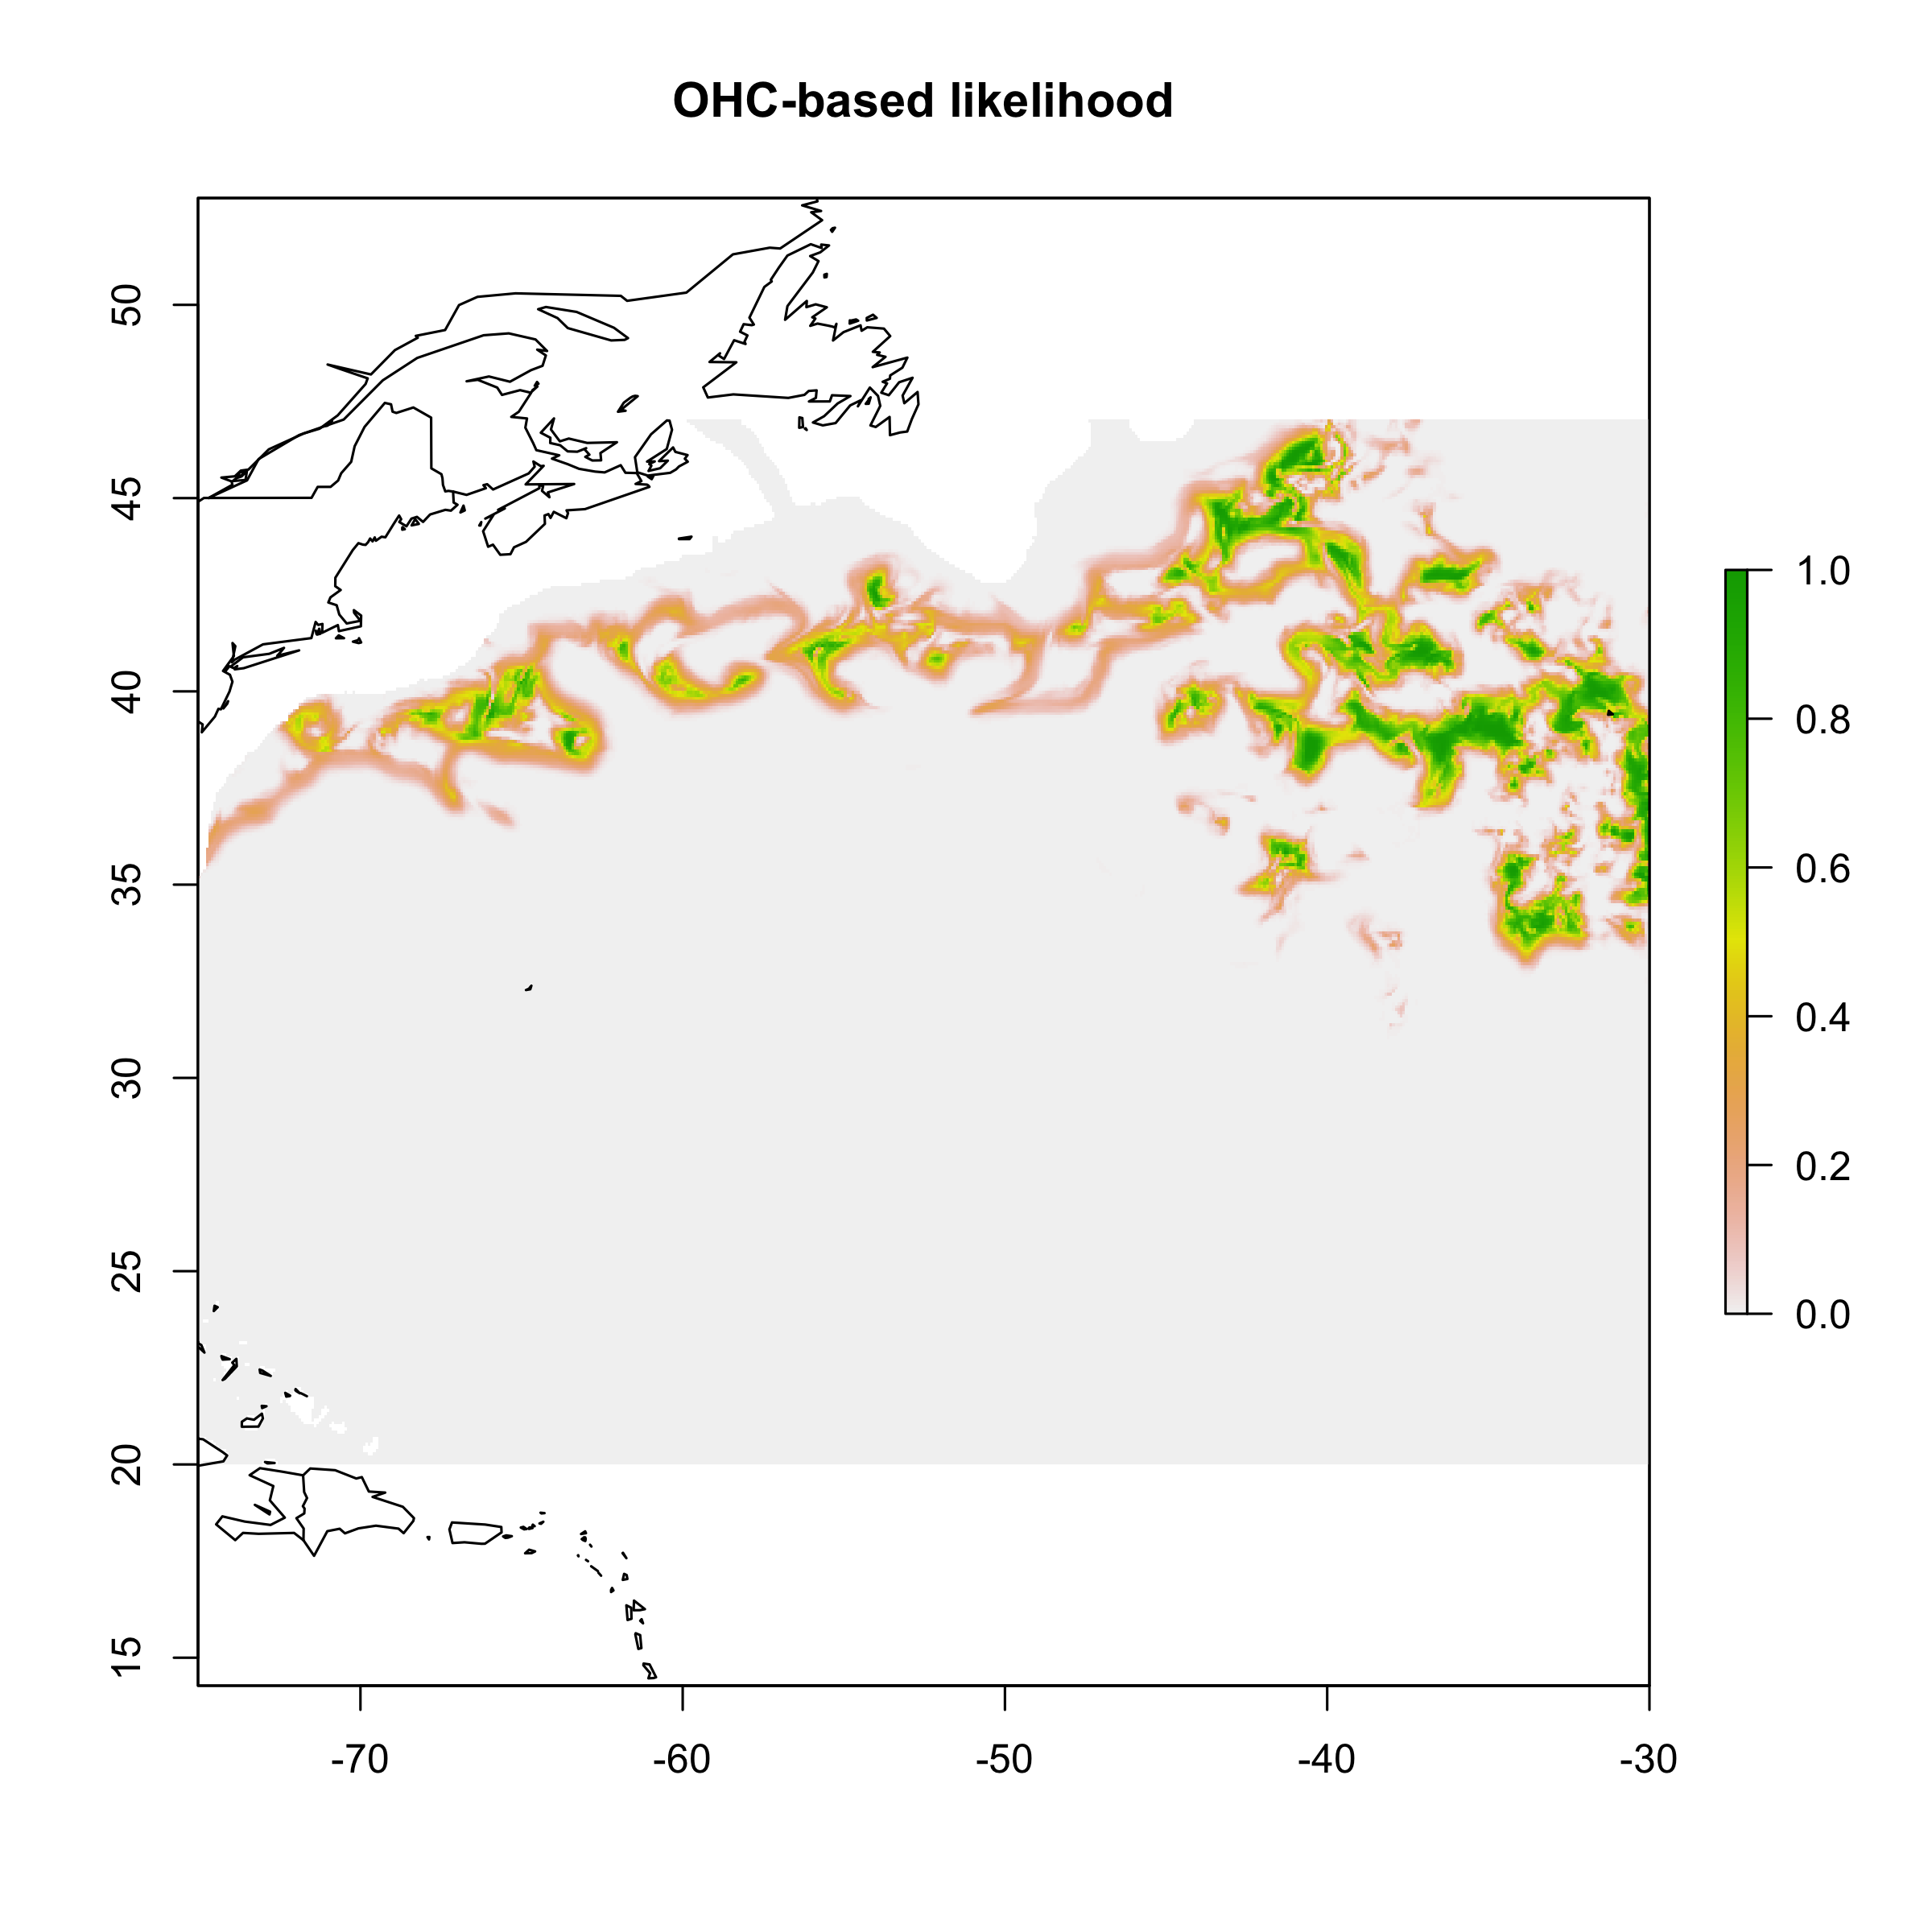
\includegraphics[width=5in, keepaspectratio]{./example_ohc_lik.png}

\begin{knitrout}\small
\definecolor{shadecolor}{rgb}{0.969, 0.969, 0.969}\color{fgcolor}\begin{kframe}
\begin{alltt}
\hlcom{# HYCOM PROFILE BASED LIKELIHOODS}
\hlstd{L.hycom} \hlkwb{<-} \hlkwd{calc.hycom}\hlstd{(pdt,} \hlkwc{filename} \hlstd{=} \hlstr{"hycom"}\hlstd{, hycom.dir,} \hlkwc{focalDim} \hlstd{=} \hlnum{9}\hlstd{,} \hlkwc{dateVec} \hlstd{=} \hlkwd{as.POSIXct}\hlstd{(dateVec),}
    \hlkwc{use.se} \hlstd{= T)}
\hlcom{## the parallel version: L.hycom <- calc.hycom.par(pdt, filename='hycom',}
\hlcom{## hycom.dir, focalDim = 9, dateVec = as.POSIXct(dateVec), use.se = T)}
\end{alltt}
\end{kframe}
\end{knitrout}

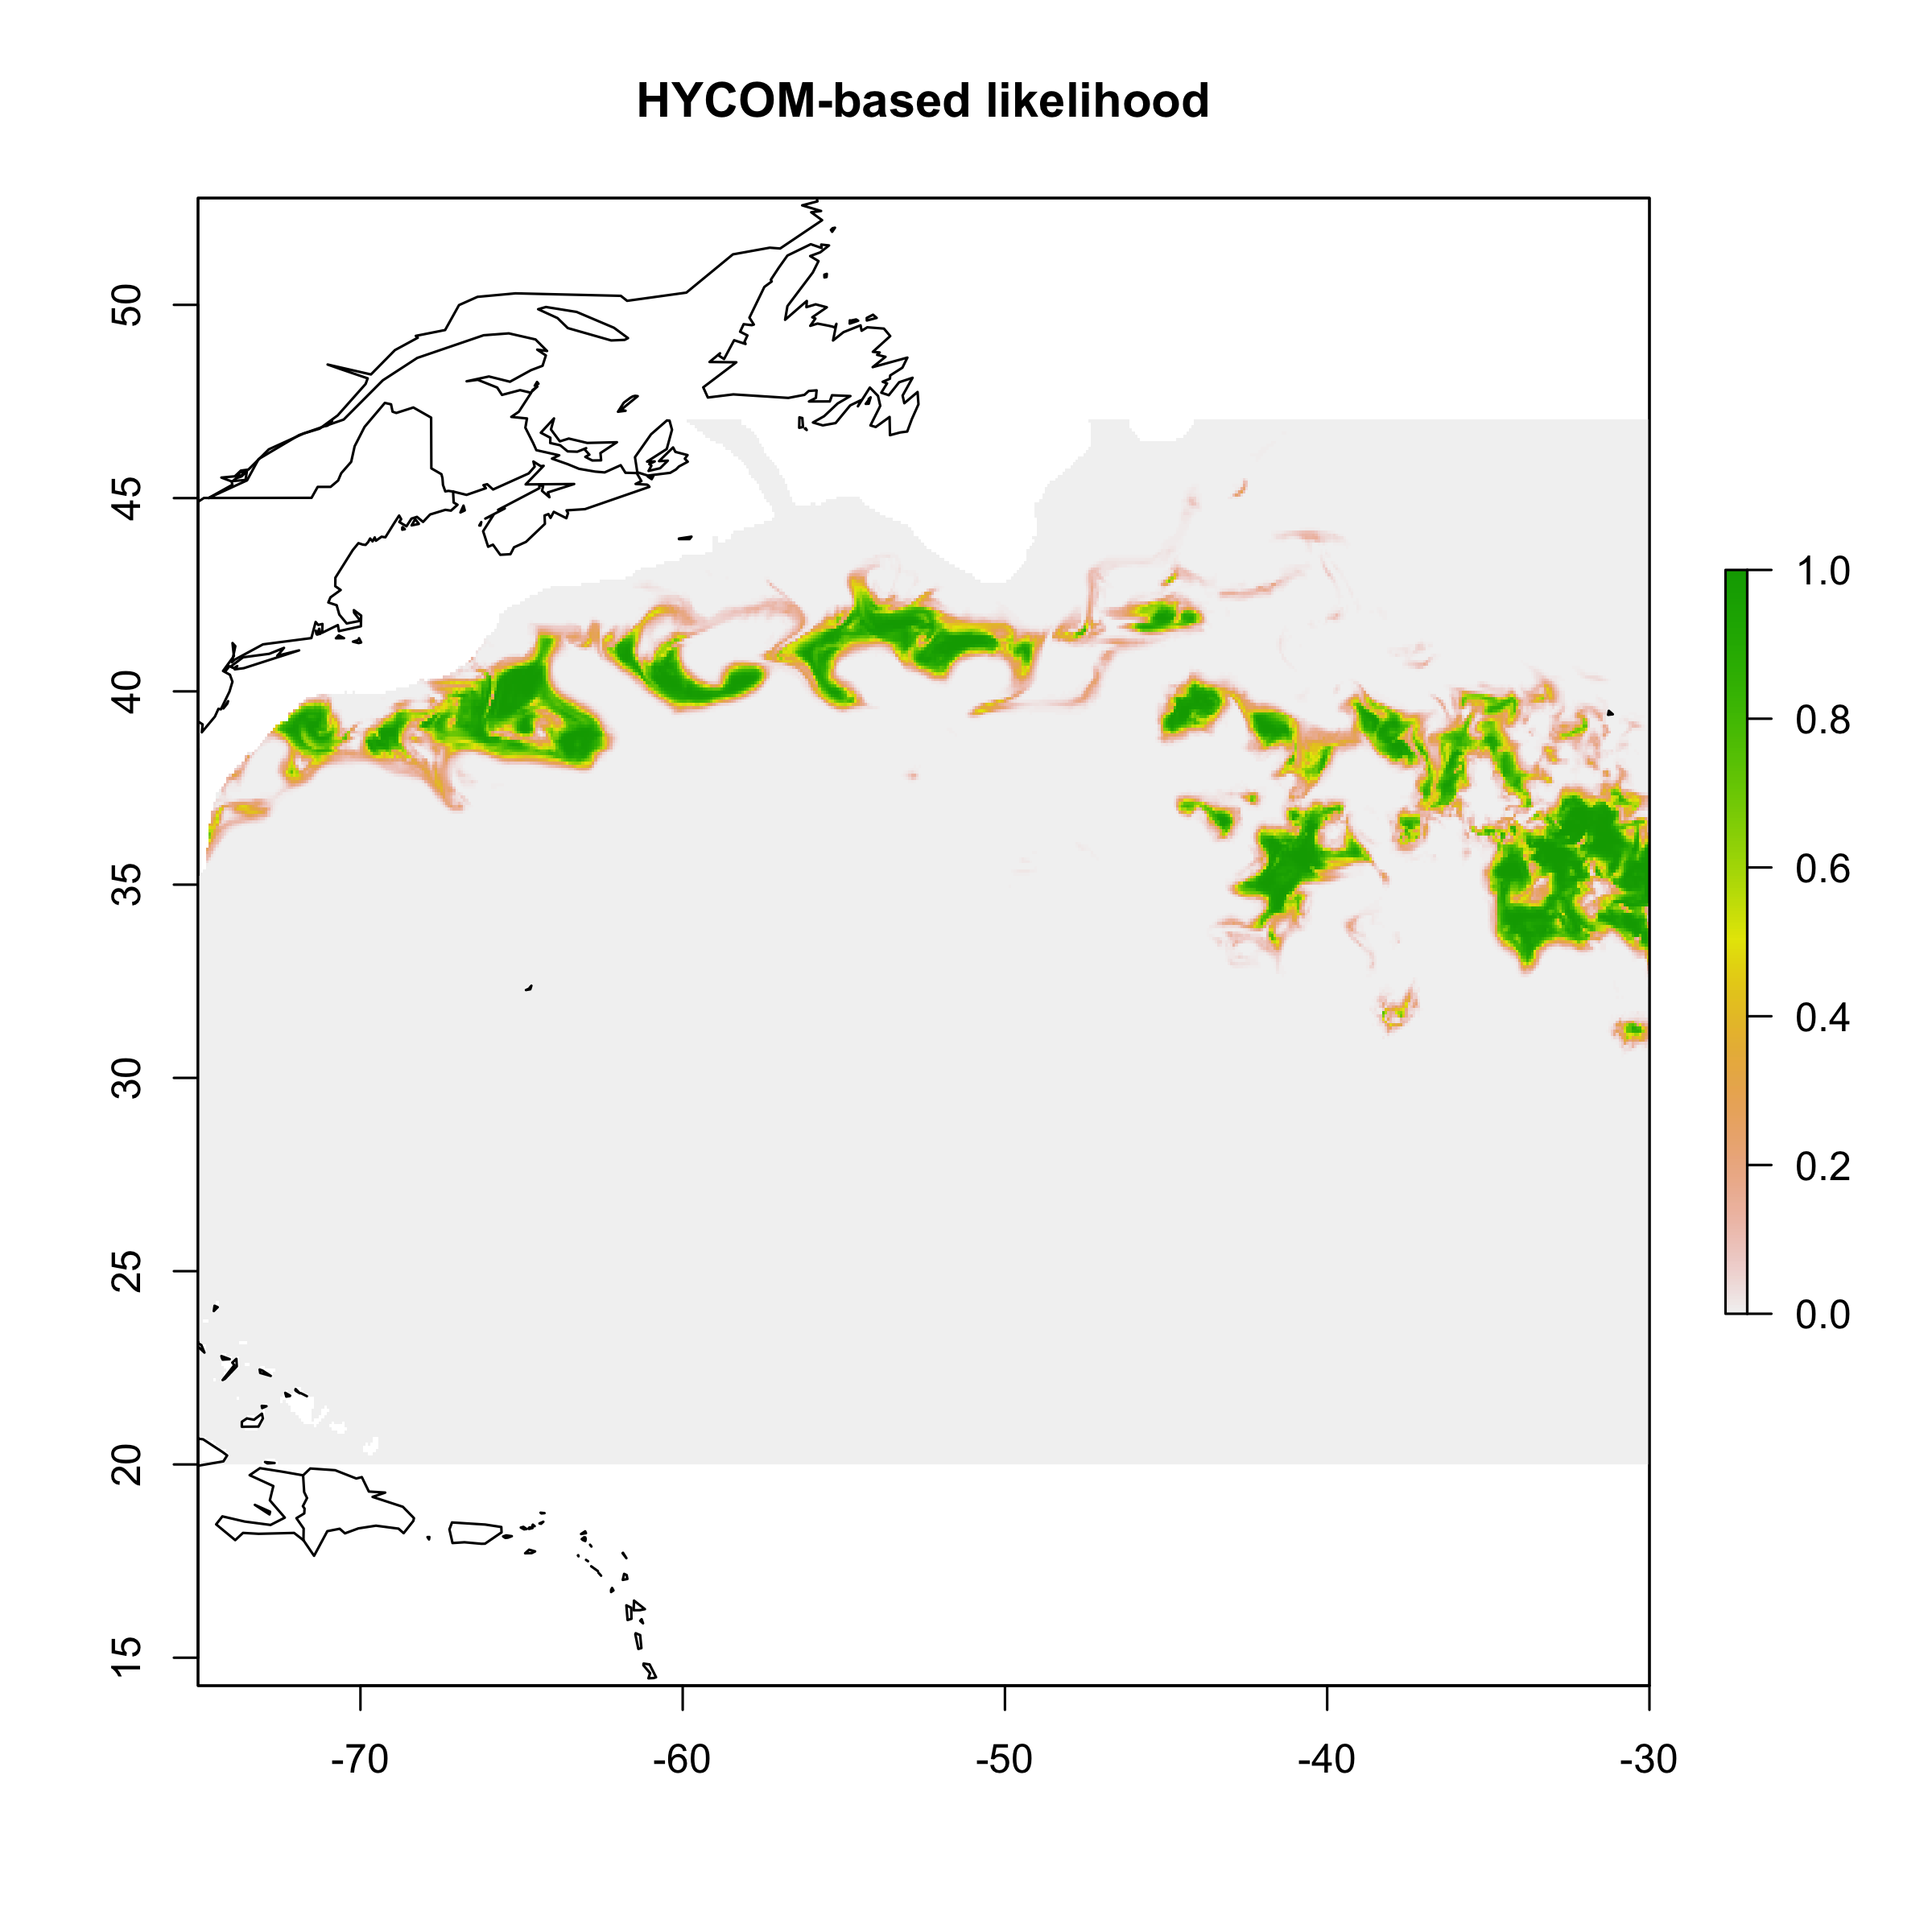
\includegraphics[width=5in, keepaspectratio]{./example_hycom_lik.png}


\subsubsection{Bathymetry likelihood}

Bathymetry can be used to further constrain the likely location of a tagged animal. The most common implementation of this is to use the maximum measured depth in each time step, compared to available bathymetry, to ensure the most probable track occupies water deep enough for the animal to make the observed vertical movements (in the implementation of \texttt{calc.bathy} this is referred to as \texttt{lik.type = 'max'}). The same approach could be used for a benthic species, but it may often make more sense for those species with reasonable certainty of interacting with the bottom to use the same approach as previous likelihoods and calculate a formal likelihood (\texttt{lik.type = 'dnorm'}). Since most bathymetry data is rather high resolution relative to the other environmental variables used here to calculate liklihoods, it usually will speed things up to down-sample the bathymetry before calculating the likelihoods. The resulting likelihood will have to be re-sampled later anyway to match other likelihood grids.

\begin{knitrout}\small
\definecolor{shadecolor}{rgb}{0.969, 0.969, 0.969}\color{fgcolor}\begin{kframe}
\begin{alltt}
\hlcom{## bathymetry based likelihood resample bathy to a more reasonable (coarse)}
\hlcom{## grid for likelihood calculations hi-res bathy grid will work but will take}
\hlcom{## longer}
\hlstd{bathy_resamp} \hlkwb{<-} \hlstd{raster}\hlopt{::}\hlkwd{resample}\hlstd{(bathy, L.sst)}  \hlcom{# or whatever grid makes sense to resample to}
\hlstd{L.bathy} \hlkwb{<-} \hlkwd{calc.bathy}\hlstd{(mmd, bathy_resamp, dateVec,} \hlkwc{focalDim} \hlstd{=} \hlnum{3}\hlstd{,} \hlkwc{sens.err} \hlstd{=} \hlnum{5}\hlstd{,}
    \hlkwc{lik.type} \hlstd{=} \hlstr{"dnorm"}\hlstd{)}
\hlstd{L.bathy} \hlkwb{<-} \hlkwd{calc.bathy.par}\hlstd{(mmd, bathy_resamp, dateVec,} \hlkwc{focalDim} \hlstd{=} \hlnum{3}\hlstd{,} \hlkwc{sens.err} \hlstd{=} \hlnum{5}\hlstd{,}
    \hlkwc{lik.type} \hlstd{=} \hlstr{"max"}\hlstd{,} \hlkwc{ncores} \hlstd{=} \hlnum{4}\hlstd{)}
\end{alltt}
\end{kframe}
\end{knitrout}

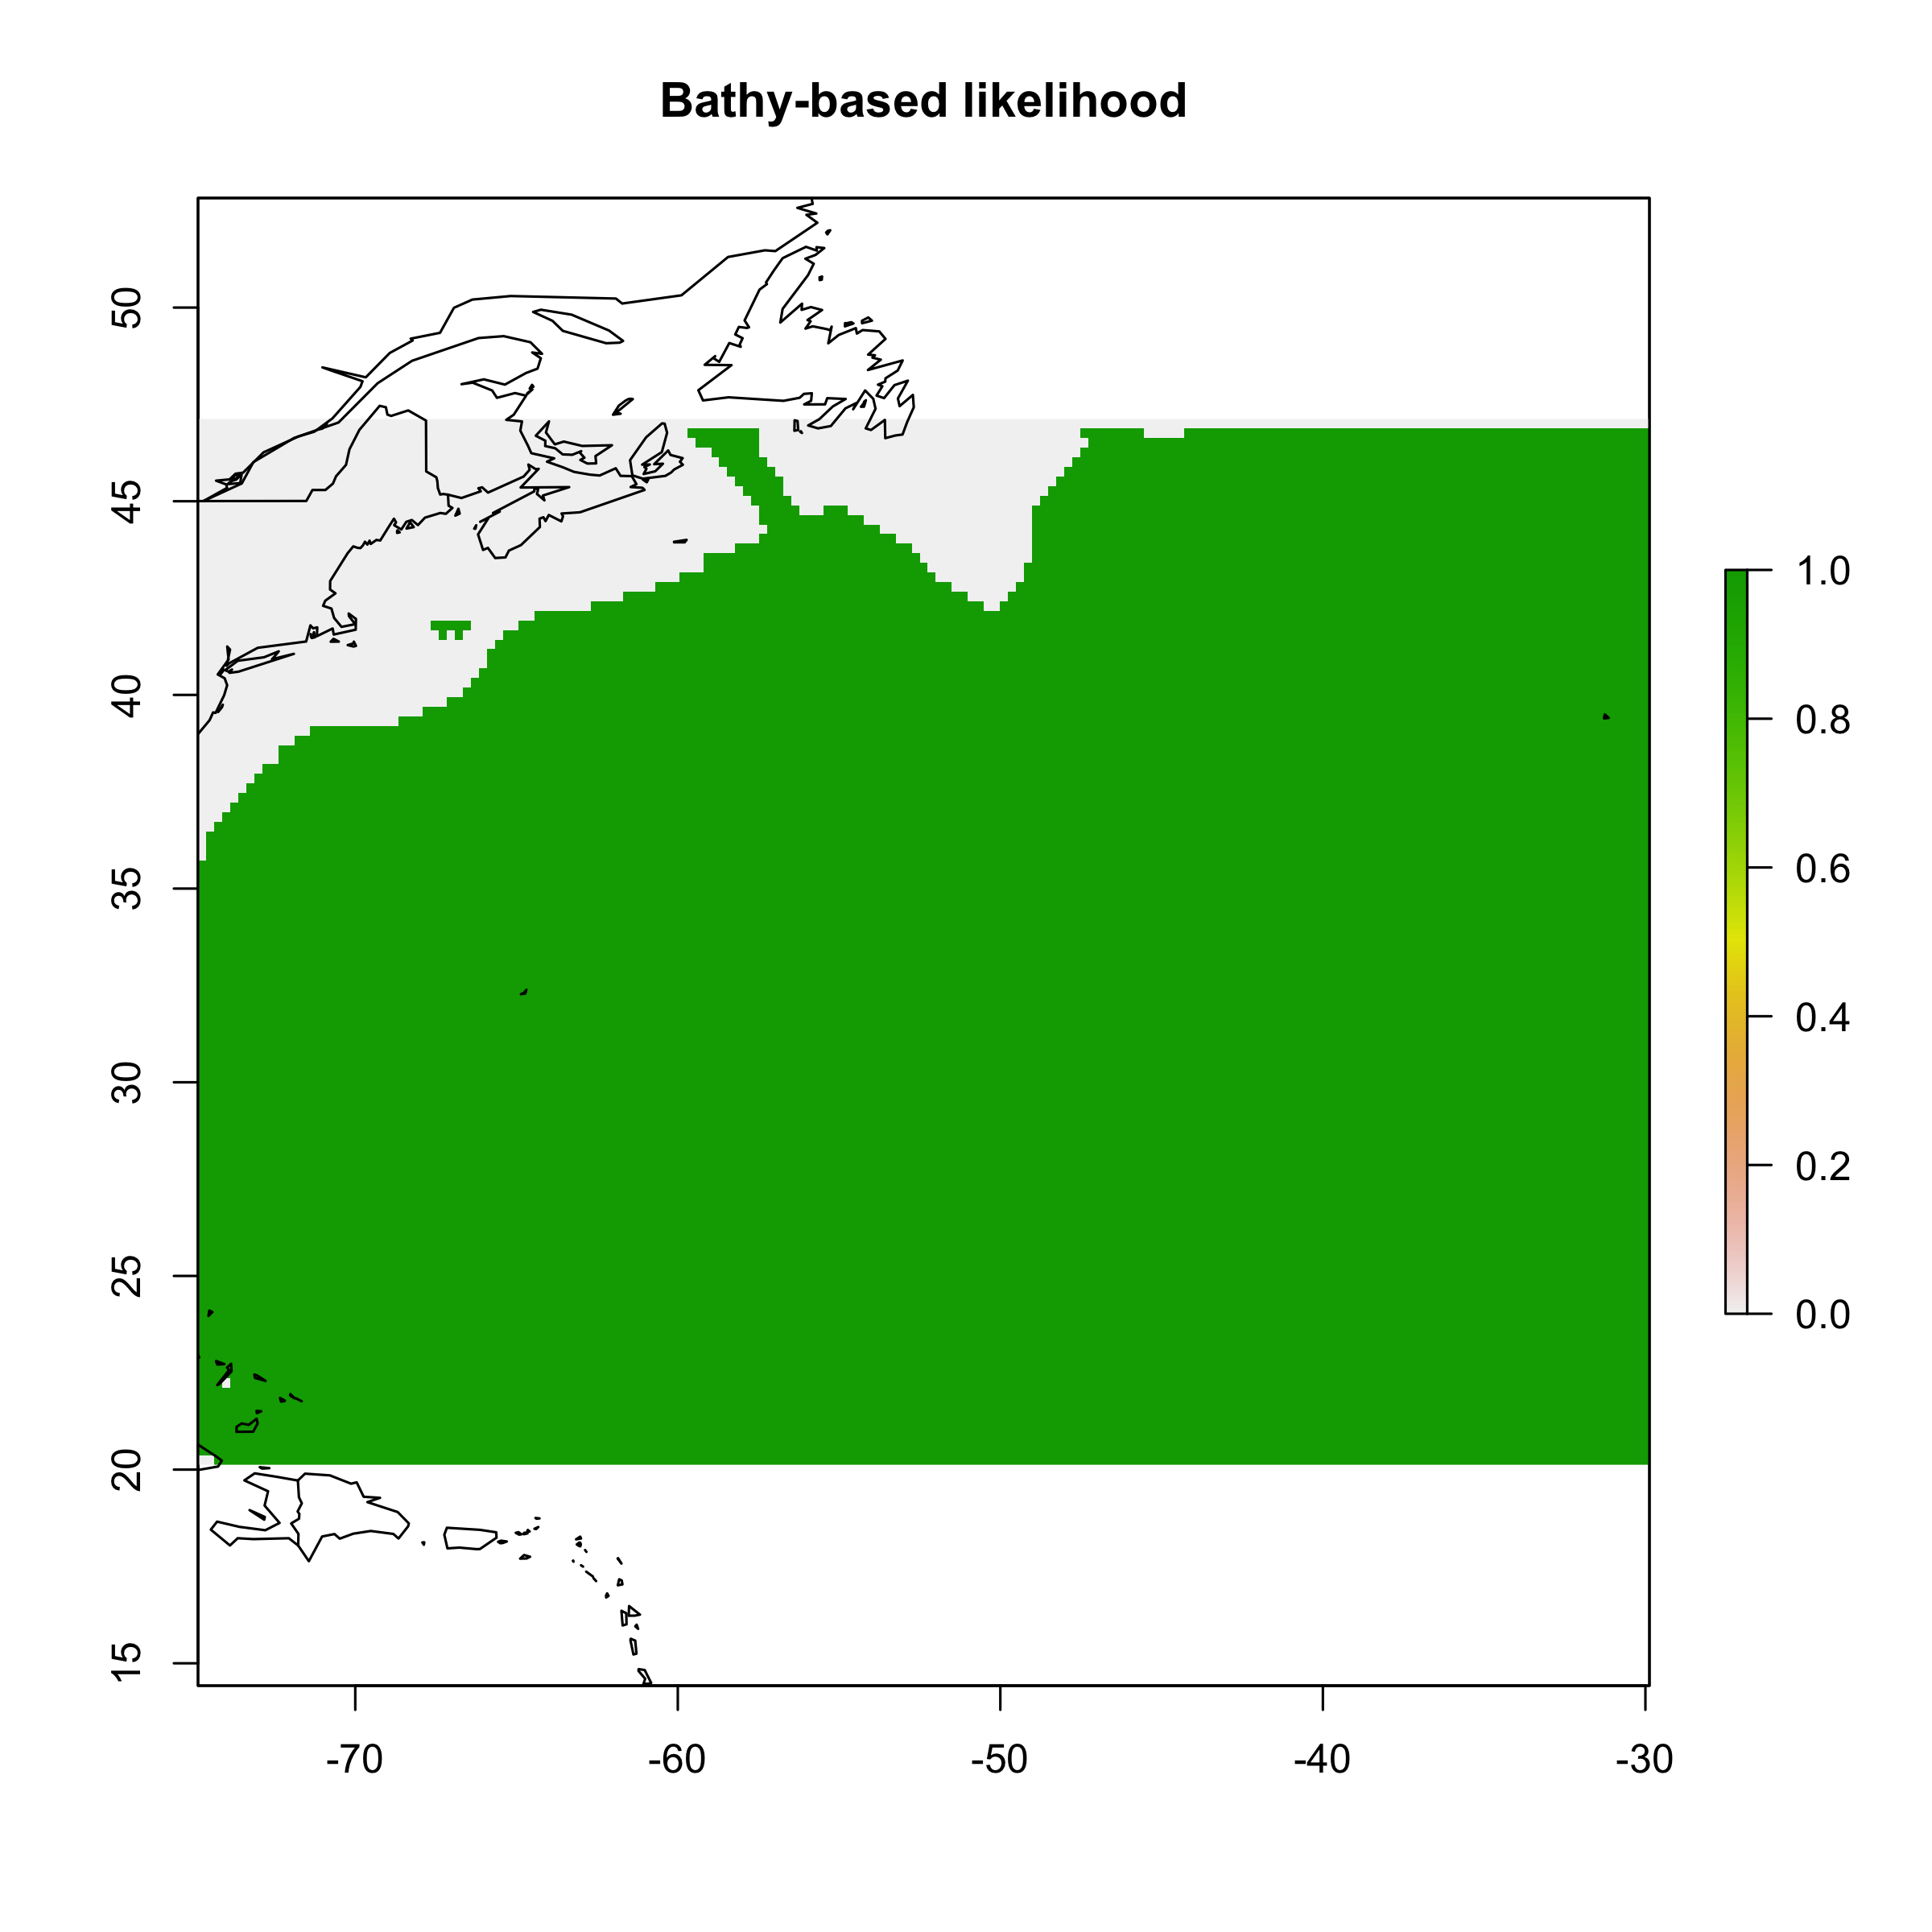
\includegraphics[width=5in, keepaspectratio]{./example_bathy_lik.png}


\subsubsection{Bottom temperature likelihood}
Gradients in bottom temperature have been used to inform geolocation of benthic species, particularly in relatively shallow and/or enclosed basins \citep[\eg cod][]{LeBris2013}. The implementation of this likelihood in \texttt{HMMoce} is similar to SST-based likelihoods but the surface temperature grid has simply been exchanged for a bottom temperature grid. Typically the environmental data for generating these likelihoods is derived from oceanographic models or some aggregate (often interpolated) set of observations.

\begin{knitrout}\small
\definecolor{shadecolor}{rgb}{0.969, 0.969, 0.969}\color{fgcolor}\begin{kframe}
\begin{alltt}
\hlcom{## bottom temperature based likelihood}
\hlstd{L.bt} \hlkwb{<-} \hlkwd{calc.bottomTemp}\hlstd{(tag.bt, dateVec,} \hlkwc{focalDim} \hlstd{=} \hlnum{3}\hlstd{,} \hlkwc{sens.err} \hlstd{=} \hlnum{1}\hlstd{,} \hlkwc{bt.dir} \hlstd{= bt.dir,}
    \hlkwc{filename} \hlstd{=} \hlstr{"bottomT"}\hlstd{,} \hlkwc{varName} \hlstd{=} \hlstr{"Temperature"}\hlstd{)}
\hlcom{# L.bt <- calc.bottomTemp.par(tag.bt, dateVec, focalDim = 3, sens.err = 1,}
\hlcom{# bt.dir = bt.dir, filename = 'bottomT', varName = 'Temperature', ncores =}
\hlcom{# 4)}
\end{alltt}
\end{kframe}
\end{knitrout}


\subsubsection{Overall observation likelihood}

The final step in generating likelihoods is to combine the likelihoods of interest to generate an overall observation-based likelihood for each time step. This is another key decision point in the geolocation process as there are a number of likelihood combinations that might make sense to base the geolocation estimates on. Here, we show just an example of one combination of likelihoods but in practice we usually iterate through multiple combinations and use a model selection approach to determine the "best" model. The final step in this section is to generate the overall observation likelihood as a combination of the selected likelihoods. At this point, you can also supply any other known locations (\eg from sightings, acoustic detections, etc).

\begin{knitrout}\small
\definecolor{shadecolor}{rgb}{0.969, 0.969, 0.969}\color{fgcolor}\begin{kframe}
\begin{alltt}
\hlcom{# COMBINE LIKELIHOOD MATRICES make list of rasters}
\hlstd{L.rasters} \hlkwb{<-} \hlkwd{list}\hlstd{(L.light, L.sst, L.ohc)}

\hlcom{## typically these will need to be resampled to have matching resolution and}
\hlcom{## extent}
\hlstd{resamp.idx} \hlkwb{<-} \hlkwd{which.max}\hlstd{(}\hlkwd{lapply}\hlstd{(L.rasters,} \hlkwc{FUN} \hlstd{=} \hlkwa{function}\hlstd{(}\hlkwc{x}\hlstd{) raster}\hlopt{::}\hlkwd{res}\hlstd{(x)[}\hlnum{1}\hlstd{]))}
\hlstd{L.res} \hlkwb{<-} \hlkwd{resample.grid}\hlstd{(L.rasters, L.rasters[[resamp.idx]])}

\hlcom{## good idea to save these likelihood rasters at some point to keep from}
\hlcom{## having to re-calculate them if (when) R crashes}

\hlcom{## finally, combine the likelihoods into a master observation likelihood that}
\hlcom{## will be used for the modeling}
\hlstd{L} \hlkwb{<-} \hlkwd{make.L}\hlstd{(ras.list, iniloc, dateVec,} \hlkwc{known.locs} \hlstd{=} \hlkwa{NULL}\hlstd{)}
\end{alltt}
\end{kframe}
\end{knitrout}

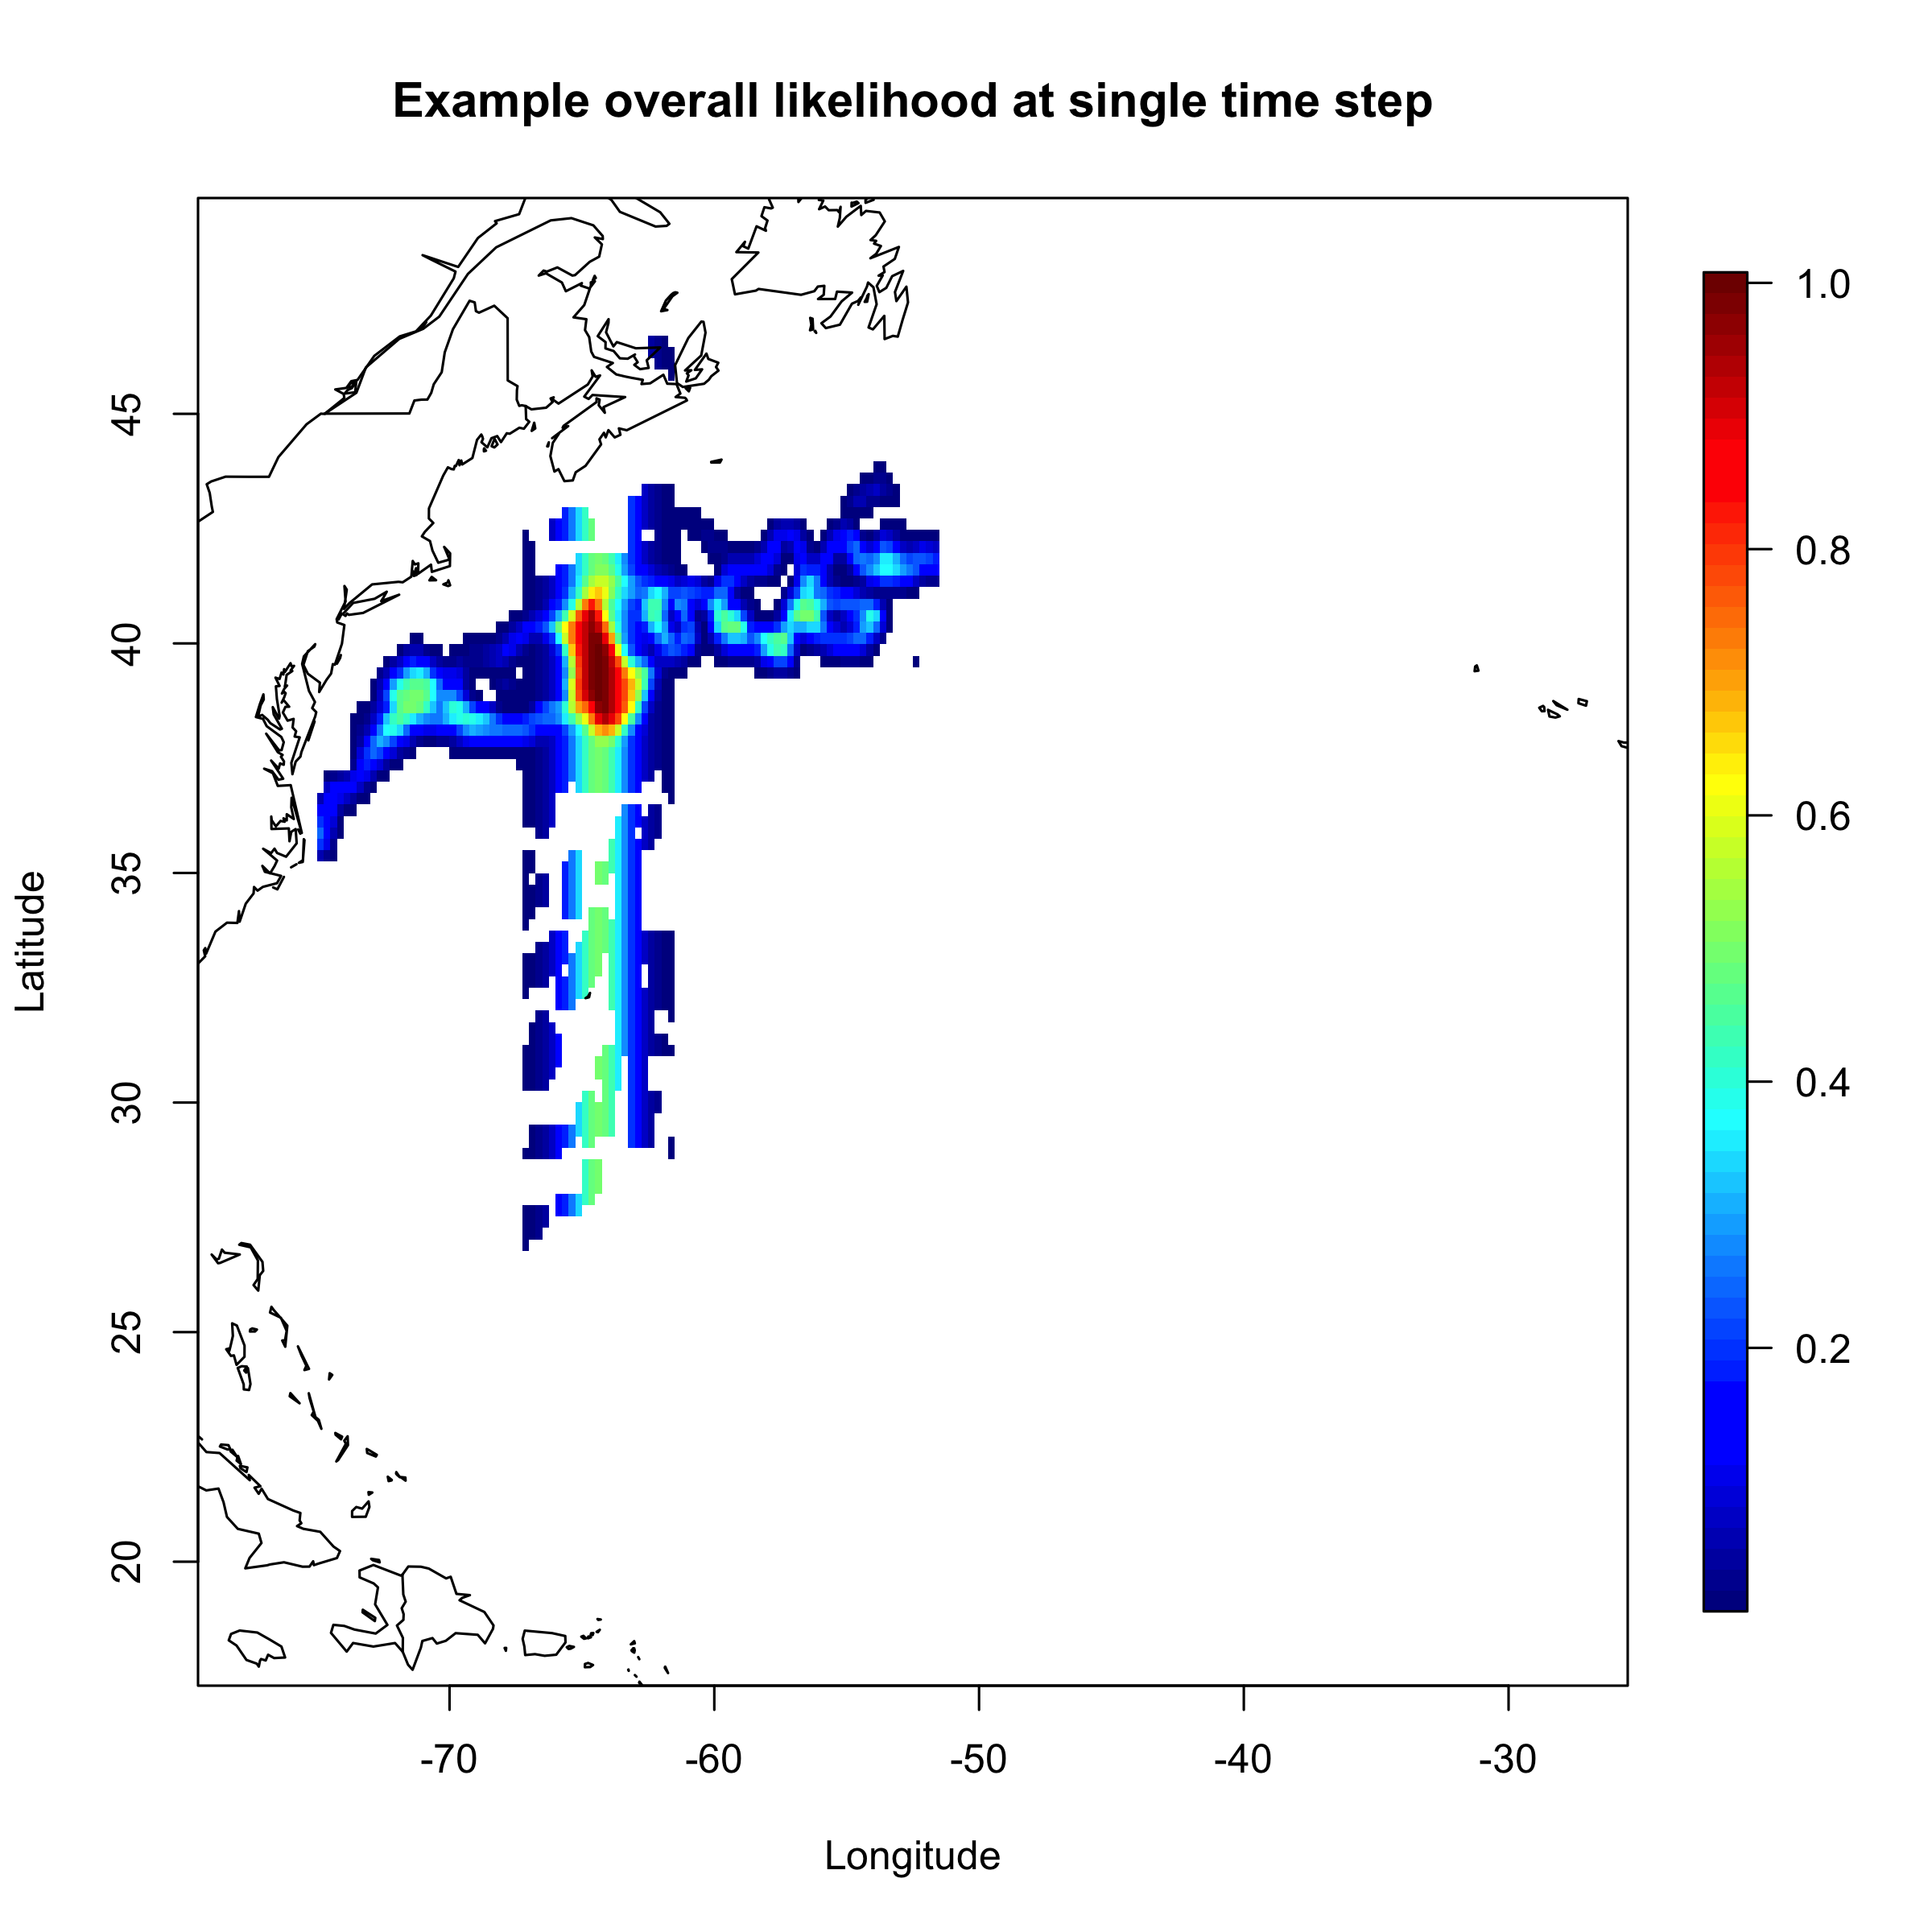
\includegraphics[width=5in, keepaspectratio]{./example_L.png}


\subsection{Model fitting}

\subsubsection{Parameter estimation}
\texttt{HMMoce} currently incorporates a handful of parameters in the HMM modeling steps. The framework currently allows 1-2 behavior states and the necessary associated parameters: diffusion or movement speed (sigmas) and state-switching probability. Obviously if only 1 behavior state is desired, state-switching probability becomes not applicable.

We currently include two general approaches to parameter estimation: gradient-based (\eg \texttt{optim}, \texttt{nlminb}) or an evolutionary / genetic algorithm. The former is faster while the latter appears to result in better estimates.

In this example, we show each of the available parameter estimation methods using a two-state model followed by one example of a single state model. In most cases, we provide upper and lower bounds on the parameters as well as initial values (the latter is not required in the genetic algorithm). Finally, parameters can be estimated much more rapidly using a more coarse grid than full resolution, however results are rarely as robust as the full resolution grids.

\begin{knitrout}\small
\definecolor{shadecolor}{rgb}{0.969, 0.969, 0.969}\color{fgcolor}\begin{kframe}
\begin{alltt}
\hlcom{## if you want to try coarse grids for parameter estimation use coarse.L()}
\hlcom{## and supply the outputs in place of L and g below}
\hlstd{L.mle} \hlkwb{<-} \hlkwd{coarse.L}\hlstd{(L, L.res}\hlopt{$}\hlstd{L.rasters)}\hlopt{$}\hlstd{L.mle}
\hlstd{g.mle} \hlkwb{<-} \hlkwd{coarse.L}\hlstd{(L, L.res}\hlopt{$}\hlstd{L.rasters)}\hlopt{$}\hlstd{g.mle}

\hlcom{## opt.params is a wrapper for the various optimization routines in HMMoce}
\hlstd{pars.optim} \hlkwb{<-} \hlkwd{opt.params}\hlstd{(}\hlkwc{pars.init} \hlstd{=} \hlkwd{c}\hlstd{(}\hlnum{2}\hlstd{,} \hlnum{0.2}\hlstd{,} \hlnum{0.6}\hlstd{,} \hlnum{0.8}\hlstd{),} \hlkwc{lower.bounds} \hlstd{=} \hlkwd{c}\hlstd{(}\hlnum{0.1}\hlstd{,}
    \hlnum{0.001}\hlstd{,} \hlnum{0.1}\hlstd{,} \hlnum{0.1}\hlstd{),} \hlkwc{upper.bounds} \hlstd{=} \hlkwd{c}\hlstd{(}\hlnum{6}\hlstd{,} \hlnum{0.6}\hlstd{,} \hlnum{0.9}\hlstd{,} \hlnum{0.9}\hlstd{),} \hlkwc{g} \hlstd{= L.res}\hlopt{$}\hlstd{g,} \hlkwc{L} \hlstd{= L,}
    \hlkwc{alg.opt} \hlstd{=} \hlstr{"optim"}\hlstd{,} \hlkwc{write.results} \hlstd{=} \hlnum{FALSE}\hlstd{)}
\hlcom{## about 22 mins on example blue shark 141259 with full grid}

\hlstd{pars.optim.mle} \hlkwb{<-} \hlkwd{opt.params}\hlstd{(}\hlkwc{pars.init} \hlstd{=} \hlkwd{c}\hlstd{(}\hlnum{2}\hlstd{,} \hlnum{0.2}\hlstd{,} \hlnum{0.6}\hlstd{,} \hlnum{0.8}\hlstd{),} \hlkwc{lower.bounds} \hlstd{=} \hlkwd{c}\hlstd{(}\hlnum{0.1}\hlstd{,}
    \hlnum{0.001}\hlstd{,} \hlnum{0.1}\hlstd{,} \hlnum{0.1}\hlstd{),} \hlkwc{upper.bounds} \hlstd{=} \hlkwd{c}\hlstd{(}\hlnum{6}\hlstd{,} \hlnum{0.6}\hlstd{,} \hlnum{0.9}\hlstd{,} \hlnum{0.9}\hlstd{),} \hlkwc{g} \hlstd{= g.mle,} \hlkwc{L} \hlstd{= L.mle,}
    \hlkwc{alg.opt} \hlstd{=} \hlstr{"optim"}\hlstd{,} \hlkwc{write.results} \hlstd{=} \hlnum{FALSE}\hlstd{)}

\hlcom{## about 1.5 mins on example blue shark 141259 with coarse grid}

\hlcom{## nlminb is also supported in HMMoce but testing suggests this is rarely the}
\hlcom{## best choice due to lack of convergence and other issues}
\hlstd{pars.nlminb} \hlkwb{<-} \hlkwd{opt.params}\hlstd{(}\hlkwc{pars.init} \hlstd{=} \hlkwd{c}\hlstd{(}\hlnum{2}\hlstd{,} \hlnum{0.2}\hlstd{,} \hlnum{0.6}\hlstd{,} \hlnum{0.8}\hlstd{),} \hlkwc{lower.bounds} \hlstd{=} \hlkwd{c}\hlstd{(}\hlnum{0.1}\hlstd{,}
    \hlnum{0.001}\hlstd{,} \hlnum{0.1}\hlstd{,} \hlnum{0.1}\hlstd{),} \hlkwc{upper.bounds} \hlstd{=} \hlkwd{c}\hlstd{(}\hlnum{5}\hlstd{,} \hlnum{0.5}\hlstd{,} \hlnum{0.9}\hlstd{,} \hlnum{0.9}\hlstd{),} \hlkwc{g} \hlstd{= L.res}\hlopt{$}\hlstd{g,} \hlkwc{L} \hlstd{= L,}
    \hlkwc{alg.opt} \hlstd{=} \hlstr{"nlminb"}\hlstd{,} \hlkwc{write.results} \hlstd{=} \hlnum{FALSE}\hlstd{)}
\hlcom{## about 30 mins on blue shark 141259}

\hlstd{pars.ga} \hlkwb{<-} \hlkwd{opt.params}\hlstd{(}\hlkwc{pars.init} \hlstd{=} \hlkwd{c}\hlstd{(}\hlnum{2}\hlstd{,} \hlnum{0.2}\hlstd{,} \hlnum{0.6}\hlstd{,} \hlnum{0.8}\hlstd{),} \hlkwc{lower.bounds} \hlstd{=} \hlkwd{c}\hlstd{(}\hlnum{0.1}\hlstd{,}
    \hlnum{0.001}\hlstd{,} \hlnum{0.1}\hlstd{,} \hlnum{0.1}\hlstd{),} \hlkwc{upper.bounds} \hlstd{=} \hlkwd{c}\hlstd{(}\hlnum{6}\hlstd{,} \hlnum{0.6}\hlstd{,} \hlnum{0.9}\hlstd{,} \hlnum{0.9}\hlstd{),} \hlkwc{g} \hlstd{= L.res}\hlopt{$}\hlstd{g,} \hlkwc{L} \hlstd{= L,}
    \hlkwc{alg.opt} \hlstd{=} \hlstr{"ga"}\hlstd{,} \hlkwc{write.results} \hlstd{=} \hlnum{FALSE}\hlstd{,} \hlkwc{ncores} \hlstd{=} \hlkwd{ceiling}\hlstd{(parallel}\hlopt{::}\hlkwd{detectCores}\hlstd{()} \hlopt{*}
        \hlnum{0.9}\hlstd{))}
\hlcom{## about 1.6 hrs on blue shark 141259 w 15 cores}

\hlstd{pars.ga.mle} \hlkwb{<-} \hlkwd{opt.params}\hlstd{(}\hlkwc{pars.init} \hlstd{=} \hlkwd{c}\hlstd{(}\hlnum{2}\hlstd{,} \hlnum{0.2}\hlstd{,} \hlnum{0.6}\hlstd{,} \hlnum{0.8}\hlstd{),} \hlkwc{lower.bounds} \hlstd{=} \hlkwd{c}\hlstd{(}\hlnum{0.1}\hlstd{,}
    \hlnum{0.001}\hlstd{,} \hlnum{0.1}\hlstd{,} \hlnum{0.1}\hlstd{),} \hlkwc{upper.bounds} \hlstd{=} \hlkwd{c}\hlstd{(}\hlnum{6}\hlstd{,} \hlnum{0.6}\hlstd{,} \hlnum{0.9}\hlstd{,} \hlnum{0.9}\hlstd{),} \hlkwc{g} \hlstd{= g.mle,} \hlkwc{L} \hlstd{= L.mle,}
    \hlkwc{alg.opt} \hlstd{=} \hlstr{"ga"}\hlstd{,} \hlkwc{write.results} \hlstd{=} \hlnum{FALSE}\hlstd{,} \hlkwc{ncores} \hlstd{=} \hlkwd{ceiling}\hlstd{(parallel}\hlopt{::}\hlkwd{detectCores}\hlstd{()} \hlopt{*}
        \hlnum{0.9}\hlstd{))}
\hlcom{## about 2 mins with MLE grid but results way different}

\hlcom{## example using the genetic algorithm and only one behavior state}
\hlstd{pars.ga.one} \hlkwb{<-} \hlkwd{opt.params}\hlstd{(}\hlkwc{pars.init} \hlstd{=} \hlkwd{c}\hlstd{(}\hlnum{2}\hlstd{),} \hlkwc{lower.bounds} \hlstd{=} \hlkwd{c}\hlstd{(}\hlnum{1}\hlstd{),} \hlkwc{upper.bounds} \hlstd{=} \hlkwd{c}\hlstd{(}\hlnum{8}\hlstd{),}
    \hlkwc{g} \hlstd{= L.res}\hlopt{$}\hlstd{g,} \hlkwc{L} \hlstd{= L,} \hlkwc{alg.opt} \hlstd{=} \hlstr{"ga"}\hlstd{,} \hlkwc{write.results} \hlstd{=} \hlnum{FALSE}\hlstd{,} \hlkwc{ncores} \hlstd{=} \hlnum{4}\hlstd{)}
\end{alltt}
\end{kframe}
\end{knitrout}

\subsubsection{HMM Filter / Smoother}

Once the parameter estimation routine(s) are finished, finalize those for input to the HMM filter/smoother. This primarily involves 1) converting movement parameters into kernels for convolution (K1/K2) and 2) converting state switching probabilities into a transition matrix (P). Once those steps are complete, everything is in place for the filter and smoother steps that generate the posterior state distributions. From that, we calculate most probable tracks by, in this case, finding the max of each posterior distribution. Other methods could be used here and may be implemented in the future (\eg Viterbi).

** explain why these values are here **


\begin{knitrout}\small
\definecolor{shadecolor}{rgb}{0.969, 0.969, 0.969}\color{fgcolor}\begin{kframe}
\begin{alltt}
\hlcom{## as an example, grab the pars from the GA using both states pars <-}
\hlcom{## pars.ga$par}

\hlcom{## or use values from a previous run as done here:}
\hlstd{pars} \hlkwb{<-} \hlkwd{c}\hlstd{(}\hlnum{4.964}\hlstd{,} \hlnum{0.217}\hlstd{,} \hlnum{0.367}\hlstd{,} \hlnum{0.484}\hlstd{)}

\hlcom{## if only one state is used in the estimation routines (above), this will}
\hlcom{## catch that here and set the parameters accordingly}
\hlkwa{if} \hlstd{(}\hlkwd{length}\hlstd{(pars)} \hlopt{==} \hlnum{4}\hlstd{) \{}
    \hlstd{sigmas} \hlkwb{=} \hlstd{pars[}\hlnum{1}\hlopt{:}\hlnum{2}\hlstd{]}
    \hlstd{sizes} \hlkwb{=} \hlkwd{rep}\hlstd{(}\hlkwd{ceiling}\hlstd{(sigmas[}\hlnum{1}\hlstd{]} \hlopt{*} \hlnum{4}\hlstd{),} \hlnum{2}\hlstd{)}
    \hlstd{pb} \hlkwb{=} \hlstd{pars[}\hlnum{3}\hlopt{:}\hlnum{4}\hlstd{]}
    \hlstd{muadvs} \hlkwb{=} \hlkwd{c}\hlstd{(}\hlnum{0}\hlstd{,} \hlnum{0}\hlstd{)}
\hlstd{\}} \hlkwa{else if} \hlstd{(}\hlkwd{length}\hlstd{(pars)} \hlopt{==} \hlnum{1}\hlstd{) \{}
    \hlstd{sigmas} \hlkwb{=} \hlstd{pars[}\hlnum{1}\hlstd{]}
    \hlstd{sizes} \hlkwb{=} \hlkwd{rep}\hlstd{(}\hlkwd{ceiling}\hlstd{(sigmas[}\hlnum{1}\hlstd{]} \hlopt{*} \hlnum{4}\hlstd{),} \hlnum{2}\hlstd{)}
    \hlstd{pb} \hlkwb{=} \hlkwa{NULL}
    \hlstd{muadvs} \hlkwb{=} \hlkwd{c}\hlstd{(}\hlnum{0}\hlstd{)}
\hlstd{\}}

\hlstd{K1} \hlkwb{<-} \hlkwd{gausskern.pg}\hlstd{(sizes[}\hlnum{1}\hlstd{], sigmas[}\hlnum{1}\hlstd{],} \hlkwc{muadv} \hlstd{= muadvs[}\hlnum{1}\hlstd{])}
\hlkwa{if} \hlstd{(}\hlopt{!}\hlkwd{is.null}\hlstd{(pb)) K2} \hlkwb{<-} \hlkwd{gausskern.pg}\hlstd{(sizes[}\hlnum{2}\hlstd{], sigmas[}\hlnum{2}\hlstd{],} \hlkwc{muadv} \hlstd{= muadvs[}\hlnum{2}\hlstd{])}

\hlkwd{image.plot}\hlstd{(K1,} \hlkwc{main} \hlstd{=} \hlstr{"Diffusion kernel for \textbackslash{}"migratory\textbackslash{}" state"}\hlstd{)}
\hlkwd{image.plot}\hlstd{(K2,} \hlkwc{main} \hlstd{=} \hlstr{"Diffusion kernel for \textbackslash{}"resident\textbackslash{}" state"}\hlstd{)}

\hlcom{# ** show kernel and how it works ** convolution?}
\end{alltt}
\end{kframe}
\end{knitrout}
 
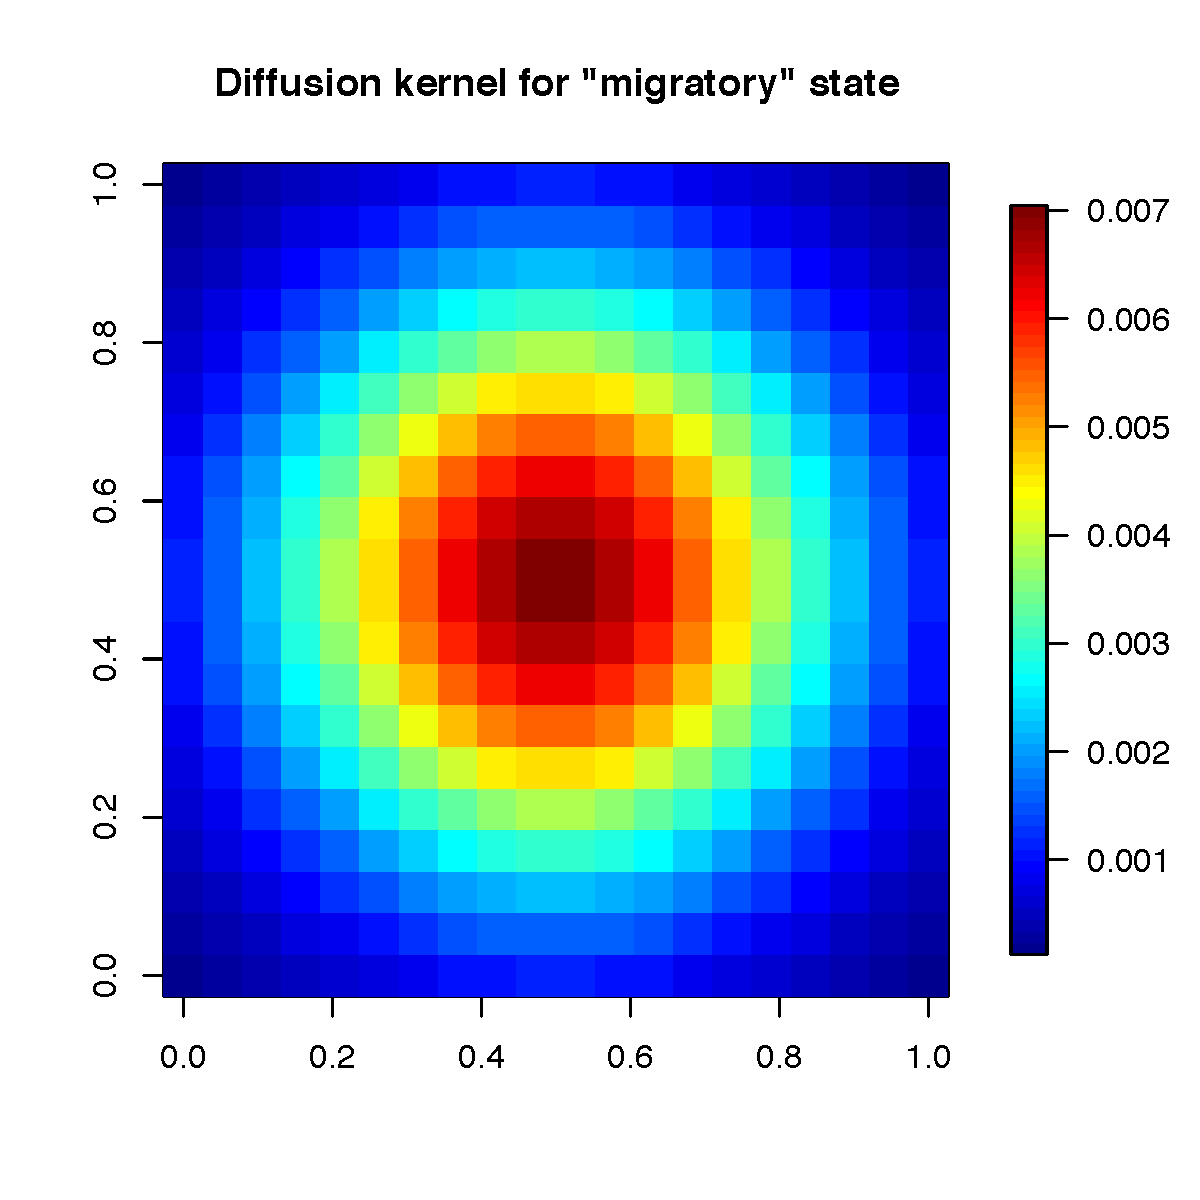
\includegraphics[width=5in, keepaspectratio]{./pars1.png}

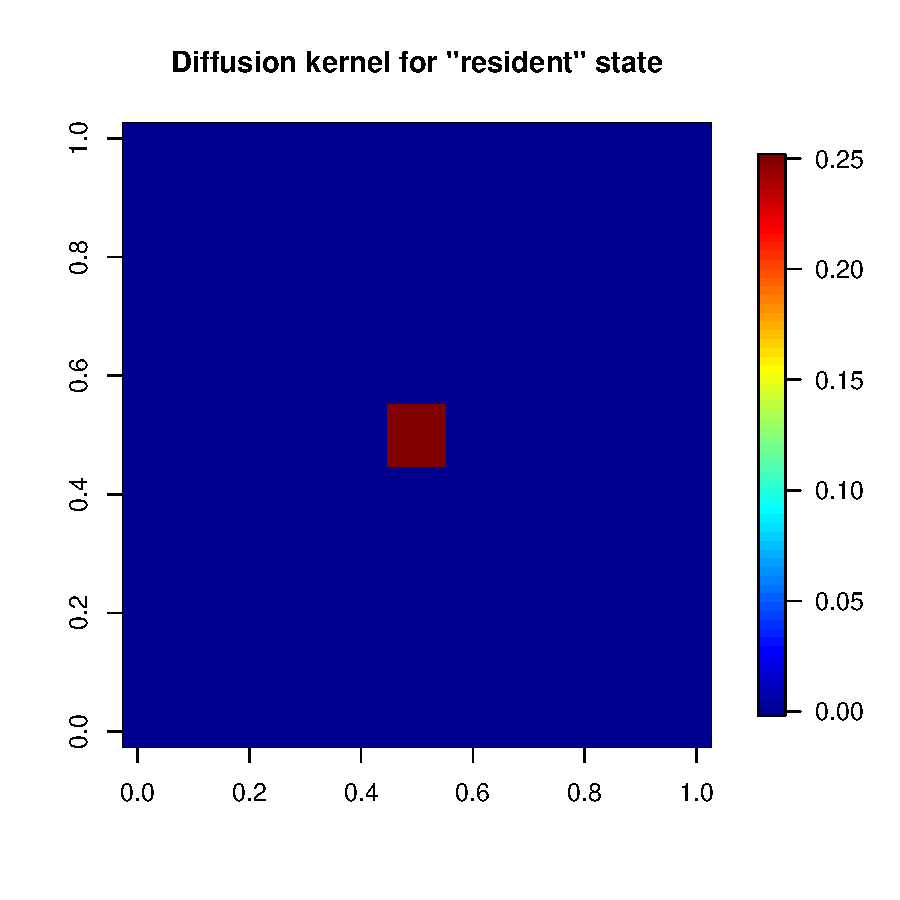
\includegraphics[width=5in, keepaspectratio]{./pars2.pdf}

\begin{knitrout}\small
\definecolor{shadecolor}{rgb}{0.969, 0.969, 0.969}\color{fgcolor}\begin{kframe}
\begin{alltt}
\hlcom{## set transition matrix, if applicable}
\hlkwa{if} \hlstd{(}\hlopt{!}\hlkwd{is.null}\hlstd{(pb)) \{}
    \hlstd{P} \hlkwb{<-} \hlkwd{matrix}\hlstd{(}\hlkwd{c}\hlstd{(pb[}\hlnum{1}\hlstd{],} \hlnum{1} \hlopt{-} \hlstd{pb[}\hlnum{1}\hlstd{],} \hlnum{1} \hlopt{-} \hlstd{pb[}\hlnum{2}\hlstd{], pb[}\hlnum{2}\hlstd{]),} \hlnum{2}\hlstd{,} \hlnum{2}\hlstd{,} \hlkwc{byrow} \hlstd{=} \hlnum{TRUE}\hlstd{)}
\hlstd{\}} \hlkwa{else} \hlstd{\{}
    \hlstd{P} \hlkwb{<-} \hlkwa{NULL}
\hlstd{\}}
\end{alltt}
\end{kframe}
\end{knitrout}


\begin{knitrout}\small
\definecolor{shadecolor}{rgb}{0.969, 0.969, 0.969}\color{fgcolor}\begin{kframe}
\begin{alltt}
\hlcom{# RUN THE FILTER STEP}
\hlkwa{if} \hlstd{(}\hlopt{!}\hlkwd{is.null}\hlstd{(pb)) \{}
    \hlstd{K} \hlkwb{<-} \hlkwd{list}\hlstd{(K1, K2)}
    \hlstd{f} \hlkwb{<-} \hlkwd{hmm.filter}\hlstd{(}\hlkwc{g} \hlstd{= L.res}\hlopt{$}\hlstd{g,} \hlkwc{L} \hlstd{= L,} \hlkwc{K} \hlstd{= K,} \hlkwc{P} \hlstd{= P,} \hlkwc{m} \hlstd{=} \hlnum{2}\hlstd{)}
\hlstd{\}} \hlkwa{else} \hlstd{\{}
    \hlstd{K} \hlkwb{<-} \hlkwd{list}\hlstd{(K1)}
    \hlstd{f} \hlkwb{<-} \hlkwd{hmm.filter}\hlstd{(}\hlkwc{g} \hlstd{= L.res}\hlopt{$}\hlstd{g,} \hlkwc{L} \hlstd{= L,} \hlkwc{K} \hlstd{= K,} \hlkwc{P} \hlstd{= P,} \hlkwc{m} \hlstd{=} \hlnum{1}\hlstd{)}
\hlstd{\}}
\hlstd{nllf} \hlkwb{<-} \hlopt{-}\hlkwd{sum}\hlstd{(}\hlkwd{log}\hlstd{(f}\hlopt{$}\hlstd{psi[f}\hlopt{$}\hlstd{psi} \hlopt{>} \hlnum{0}\hlstd{]))}  \hlcom{# negative log-likelihood}
\hlstd{AIC} \hlkwb{<-} \hlnum{2} \hlopt{*} \hlstd{nllf} \hlopt{+} \hlnum{2} \hlopt{*} \hlkwd{length}\hlstd{(}\hlkwd{which}\hlstd{(}\hlopt{!}\hlkwd{is.na}\hlstd{(pars)))}

\hlcom{# RUN THE SMOOTHING STEP}
\hlstd{s} \hlkwb{<-} \hlkwd{hmm.smoother}\hlstd{(f,} \hlkwc{K} \hlstd{= K,} \hlkwc{L} \hlstd{= L,} \hlkwc{P} \hlstd{= P)}

\hlcom{# GET THE MOST PROBABLE TRACK AS MEAN OF POSTERIOR DISTRIBUTION OF STATE}
\hlstd{tr} \hlkwb{<-} \hlkwd{calc.track}\hlstd{(s,} \hlkwc{g} \hlstd{= L.res}\hlopt{$}\hlstd{g, dateVec, iniloc,} \hlkwc{method} \hlstd{=} \hlstr{"mean"}\hlstd{)}
\end{alltt}
\end{kframe}
\end{knitrout}

\subsubsection{Plotting results}

\begin{knitrout}\small
\definecolor{shadecolor}{rgb}{0.969, 0.969, 0.969}\color{fgcolor}\begin{kframe}
\begin{alltt}
\hlkwd{plotHMM}\hlstd{(s, tr, dateVec,} \hlkwc{ptt} \hlstd{=} \hlstr{"141259_example"}\hlstd{,} \hlkwc{save.plot} \hlstd{= F)}

\hlcom{# plotRD(s, tr, ptt='141259_example', g = g, xlims = c(sp.lim$xmin,}
\hlcom{# sp.lim$xmax), ylims = c(sp.lim$ymin, sp.lim$ymax), makePlot = TRUE,}
\hlcom{# save.plot=FALSE)}
\end{alltt}
\end{kframe}
\end{knitrout}


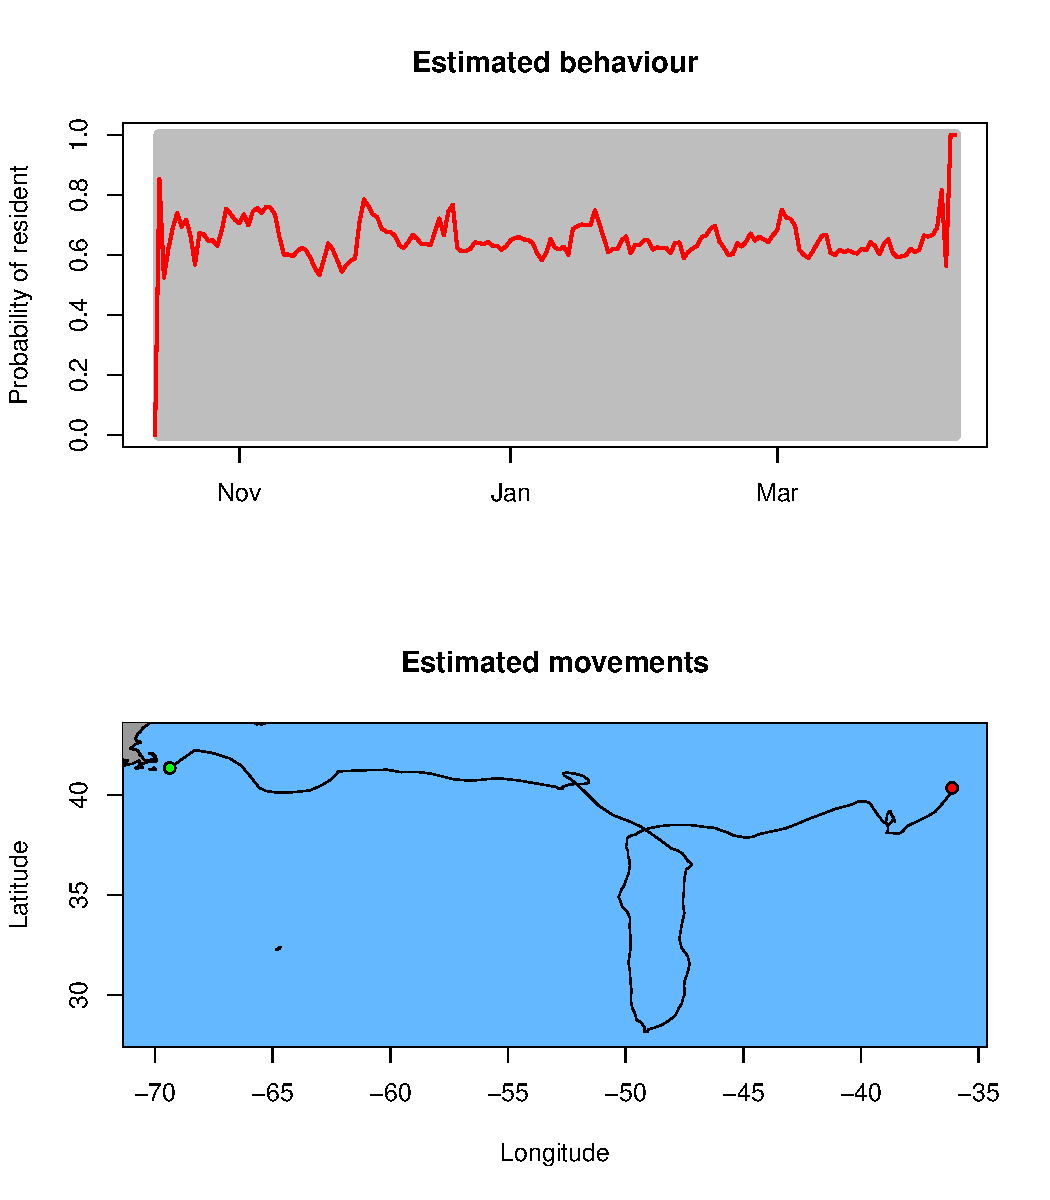
\includegraphics[width=5in, keepaspectratio]{./141259_example_track_results.pdf}


%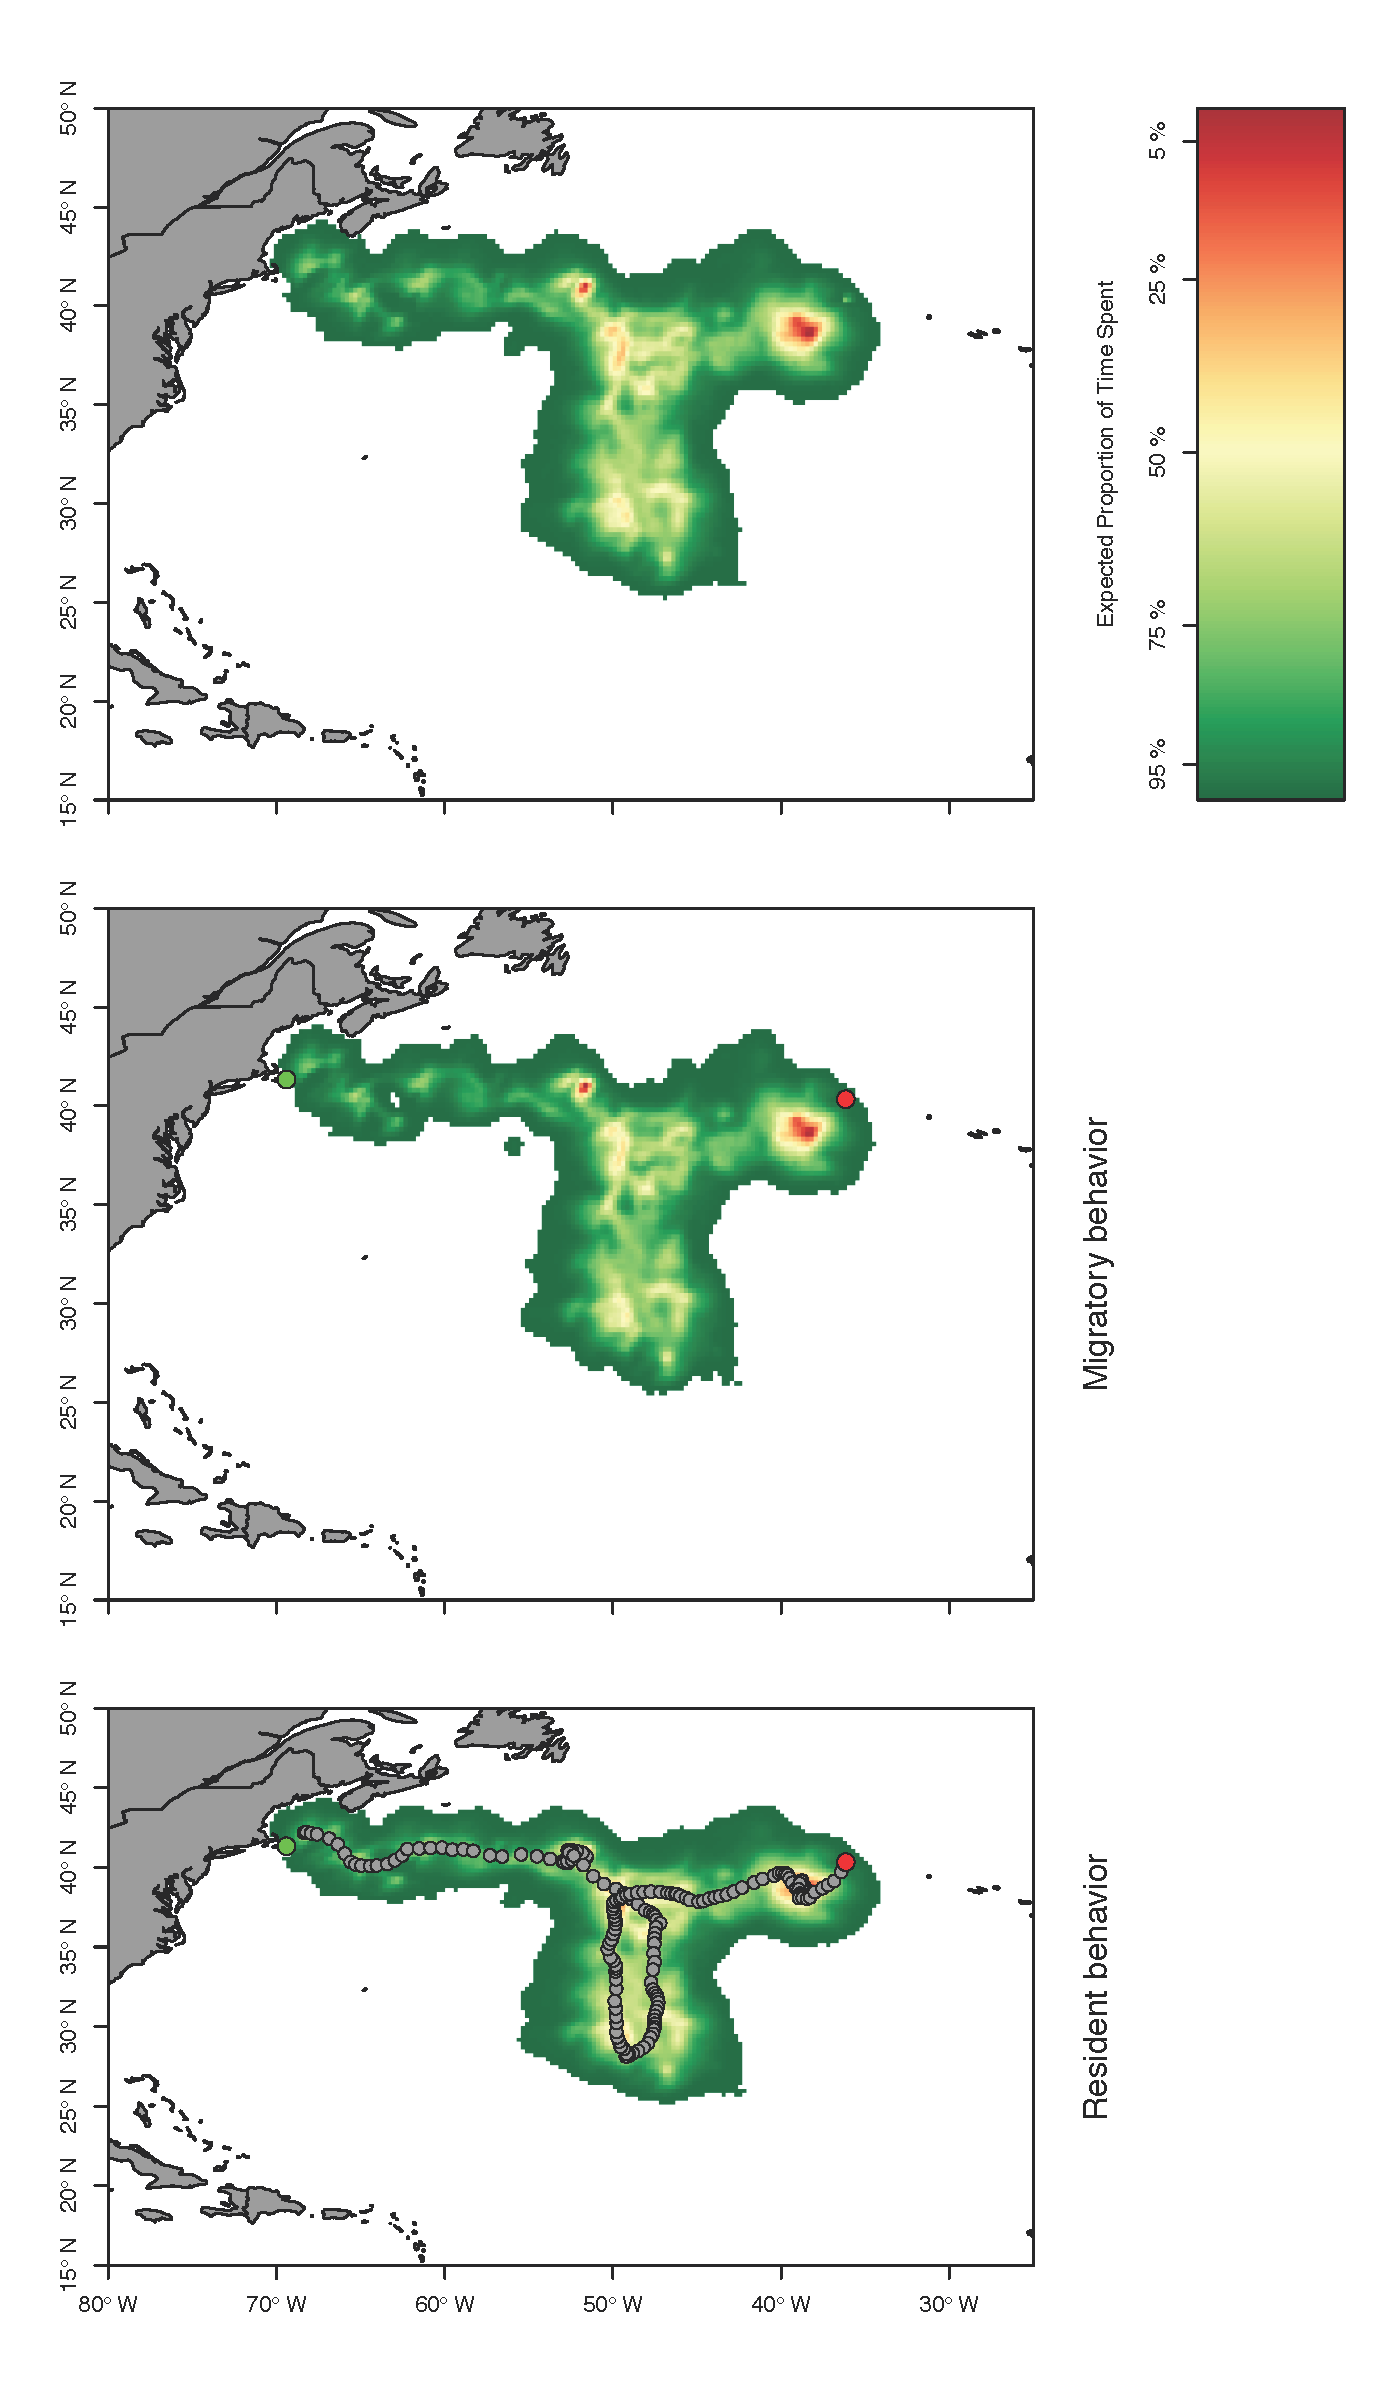
\includegraphics[width=5in, keepaspectratio]{./figure/141259_example_RD.png}



\subsubsection{Comparing models and selection}

Info here on NLL/AIC and model scoring


\subsection{Resources}

While the above is a nice simple introduction to \texttt{HMMoce} using 1 example tag dataset, rarely are we running only 1 model and for just a single individual. Often we want to iterate through a bunch of different potential likelihood combinations and parameters (\ie 1 state vs 2). Comparing and selecting models is covered above, but some "real world" example run scripts may also be helpful to show how we might tackle applying this model framework to multiple datasets for a given study, for example.

Here's an example run script for a set of bigeye tuna tagged with Microwave X-tags:
\url{https://github.com/camrinbraun/HMMoce_run/blob/master/run_GoletBET.r}

Here's an example run script for a handful of porbeagle tagged with PSATs, some of which were physically recovered:
\url{https://github.com/camrinbraun/HMMoce_run/blob/master/run_porbeagle_archival.r}

Note that the Github repo (\url{https://github.com/camrinbraun/HMMoce_run}) where a lot of these run scripts live is messy and contains many outdated (likely disfunctional) scripts. The best resources will be the newest or most recently modified such as those linked above.

\bibliographystyle{apalike}
\bibliography{hmm_ms}

\end{document}
